% !TeX program = xelatex
% 详细中文 Beamer 汇报。请使用 XeLaTeX 编译两次。
\documentclass[aspectratio=169,11pt]{beamer}
\usepackage[UTF8,fontset=fandol]{ctex}
\usepackage{amsmath,amssymb,booktabs,array,tabularx,graphicx}
\usepackage{pgfplots}
\pgfplotsset{compat=1.18}
\usetikzlibrary{arrows.meta,positioning,calc}
% 已确认的经典蓝色 Madrid 主题
\usetheme{Madrid}
\usefonttheme{professionalfonts}
\definecolor{AcademicBlue}{RGB}{51,51,178}
\definecolor{BlueDark}{RGB}{26,26,89}
\definecolor{BlueMid}{RGB}{38,38,134}
\definecolor{NoteGray}{RGB}{105,105,105}
\definecolor{GridGray}{RGB}{220,220,230}
\setbeamercolor{structure}{fg=AcademicBlue}
\setbeamercolor{palette primary}{fg=white,bg=AcademicBlue}
\setbeamercolor{palette secondary}{fg=white,bg=BlueMid}
\setbeamercolor{palette tertiary}{fg=white,bg=BlueDark}
\setbeamercolor{frametitle}{fg=white,bg=AcademicBlue}
\setbeamercolor{title}{fg=white,bg=AcademicBlue}
\setbeamercolor{subtitle}{fg=white}
\setbeamercolor{normal text}{fg=black,bg=white}
\setbeamercolor{block title}{fg=white,bg=AcademicBlue}
\setbeamercolor{block body}{fg=black,bg=AcademicBlue!7!white}
\setbeamercolor{author in head/foot}{fg=white,bg=BlueDark}
\setbeamercolor{title in head/foot}{fg=white,bg=BlueMid}
\setbeamercolor{date in head/foot}{fg=white,bg=AcademicBlue}
\setbeamerfont{title}{size=\Large,series=\mdseries}
\setbeamerfont{subtitle}{size=\normalsize,series=\mdseries}
\setbeamerfont{frametitle}{size=\Large,series=\mdseries}
\setbeamerfont{block title}{size=\normalsize,series=\mdseries}
\setbeamerfont{author}{size=\normalsize}
\setbeamerfont{institute}{size=\small}
\setbeamerfont{date}{size=\normalsize}
\setbeamersize{text margin left=5mm,text margin right=5mm}
\setbeamertemplate{navigation symbols}{}
\setbeamertemplate{headline}{}
\setbeamertemplate{enumerate items}[ball]
\setbeamertemplate{items}[ball]
\setbeamertemplate{blocks}[rounded][shadow=true]
% 部分旧版PGF的dvipdfmx驱动在保存阴影对象编号时使用了错误的let展开。
% 下方仅对具有该对象计数器的dvipdfmx类后端应用等价的资源登记定义。
\makeatletter
\AtBeginDocument{%
  \@ifundefined{pgfsys@objnum}{}{%
    \def\pgf@sys@pdf@install@mask#1{%
      \pgfutil@addpdfresource@extgs{%
        /pgfsmask\csname pgfsmaskxform@#1\endcsname\space <<
        /SMask << /S /Luminosity /G @pgfsmask\csname pgfsmaskxform@#1\endcsname >> >>}%
      \expandafter\xdef\csname pgfsmask@#1\endcsname{\csname pgfsmaskxform@#1\endcsname}%
    }%
  }%
}
\makeatother
\setlength{\parindent}{0pt}
\setbeamertemplate{footline}{%
  \leavevmode\hbox{%
  \begin{beamercolorbox}[wd=.25\paperwidth,ht=2.1ex,dp=.85ex,center]{author in head/foot}%
    \fontsize{5}{6}\selectfont\bfseries\insertshortauthor\quad 空间转录组学入门
  \end{beamercolorbox}%
  \begin{beamercolorbox}[wd=.416666\paperwidth,ht=2.1ex,dp=.85ex,center]{title in head/foot}%
    \fontsize{5}{6}\selectfont\bfseries\insertsubsectionhead
  \end{beamercolorbox}%
  \begin{beamercolorbox}[wd=.333334\paperwidth,ht=2.1ex,dp=.85ex]{date in head/foot}%
    \fontsize{5}{6}\selectfont\bfseries\hspace{5mm}\insertshortdate
    \hfill\insertframenumber\,/\,\inserttotalframenumber\hspace{1.5mm}
  \end{beamercolorbox}}}
\hypersetup{colorlinks=true,urlcolor=NoteGray,linkcolor=white,citecolor=NoteGray}
\newcommand{\source}[1]{\vfill\par{\fontsize{6}{8}\selectfont\color{NoteGray}\raggedright #1\par}}
\newcommand{\teaching}{\source{教学构造：沿用原讲义示例，不是真实实验数据。}}
\newcommand{\bluelabel}[1]{{\color{AcademicBlue}#1}\par\smallskip}
\newcommand{\keypoint}[2]{\begin{block}{#1}#2\end{block}}
\newcommand{\wideitems}{\setlength{\itemsep}{.75em}}
\newcommand{\compactitems}{\setlength{\itemsep}{.35em}}
\newcolumntype{Y}{>{\raggedright\arraybackslash}X}
\newcommand{\codetext}[1]{\texttt{#1}}

\title[空间转录组学入门]{空间转录组学入门}
\subtitle{从细胞与分子到数据分析与科研验证\\面向计算机与人工智能专业的详细汇报}
\author[Auutuumn]{Auutuumn}
\institute{面向 CS / AI 背景的本科生与研究生}
\date[2026年10月21日]{2026年10月21日}
\hypersetup{pdftitle={空间转录组学入门：详细学术汇报},pdfauthor={Auutuumn}}
\setbeameroption{hide notes}
\begin{document}
% PAGE 1 / 空间转录组学入门
\begin{frame}\relax
\titlepage
\note{开场说明受众：这是一场面向计算机和人工智能背景同学的入门汇报。先建立生物学直觉，再读懂数据，最后讨论模型输出能支持怎样的科学结论。}
\end{frame}

% PAGE 2 / 学习目标与汇报范围
\begin{frame}{学习目标与汇报范围}\relax
\begin{itemize}\wideitems
\item 解释细胞、DNA、RNA、蛋白质与基因表达的关系。
\item 说清空间转录组测什么，以及为什么需要保留位置。
\item 读懂表达矩阵、空间坐标和组织图像的对应关系。
\item 把生物问题翻译成算法任务，并判断结果需要怎样验证。
\end{itemize}
\note{不要求提前学过分子生物学。提醒听众不用一次背下全部名词，关键是知道每个名词在证据链中扮演什么角色。后面的公式用于解释数据，不是以数学复杂度为目标。}
\end{frame}

% PAGE 3 / 汇报主线与章节安排
\begin{frame}{汇报主线与章节安排}\relax
\par\noindent{\small\setlength{\tabcolsep}{7pt}\renewcommand{\arraystretch}{1.3}
\begin{tabularx}{\dimexpr\linewidth-4pt\relax}{@{}YYY@{}}\toprule
部分 & 原讲义章节 & 本部分的问题\\\midrule
一、生物学基础 & 第1--5章 & 我们研究什么，RNA为什么能提供信息？\\
二、测量与空间信息 & 第6--9章 & 怎样测量，如何保留位置？\\
三、计算与科研验证 & 第10--15章 & 怎样表示、分析并验证数据？\\
四、术语与延伸阅读 & 第16--17章 & 怎样回查概念并继续学习？\\
\bottomrule\end{tabularx}\par}

\note{说明四部分的递进关系：分子与细胞决定我们测什么，实验决定数据含义，数据决定可做的任务，验证设计决定结论边界。章节顺序与讲义一致。}
\end{frame}

% PAGE 4 / 贯穿全篇的例子：肿瘤组织薄片
\begin{frame}{贯穿全篇的例子：肿瘤组织薄片}\relax
\begin{itemize}\wideitems
\item 研究材料：一张含多种细胞的肿瘤组织切片。
\item 研究问题：免疫细胞主要分布在肿瘤内部，还是边缘？
\item 需要的信息：表达信号、真实位置、组织区域与验证依据。
\end{itemize}\keypoint{先保留一个问题}{从RNA信号到“免疫细胞在哪里”，中间需要哪些推断？}
\note{明确这是研究问题示例，不预设免疫细胞一定出现在某个区域。后续计数是教学构造，也不会凭分布直接推断治疗效果。请听众带着“哪些是测到的，哪些是推出来的”这条问题线继续。}
\end{frame}

\section{第一部分：生物学基础}

% PAGE 5 / 第一部分：生物学基础
\begin{frame}{第一部分：生物学基础}\relax
\keypoint{核心问题}{细胞怎样保存和使用信息，RNA为什么能帮助描述细胞？}\begin{itemize}\wideitems
\item 第1--2章：组织、细胞、DNA与基因。
\item 第3--4章：转录、RNA、翻译与蛋白质。
\item 第5章：表达组合、细胞身份与细胞状态。
\end{itemize}
\note{先把研究对象建立起来。提醒听众类比有助于入门，但类比不是对真实分子过程的完整解释。}
\end{frame}

\subsection{第1章：组织和细胞}

% PAGE 6 / 第1章：组织和细胞
\begin{frame}{第1章：组织和细胞}\relax
\vfill\begin{center}\begin{minipage}{.86\linewidth}
{\large\color{AcademicBlue}本章导读\par}\vspace{4mm}
{\Large 本章先认识组织与细胞的层次、基本结构和形态信息。\par\vspace{4mm}这些概念帮助我们理解，空间转录组中的信号来自怎样的研究对象。\par}
\end{minipage}\end{center}\vfill
\source{依据：配套讲义第1章。}
\note{章节导入。本章先认识组织与细胞的层次、基本结构和形态信息。这些概念帮助我们理解，空间转录组中的信号来自怎样的研究对象。}
\end{frame}

% PAGE 7 / 组织与细胞的层次
\begin{frame}{组织与细胞的层次}\relax
\par\noindent{\small\setlength{\tabcolsep}{7pt}\renewcommand{\arraystretch}{1.3}
\begin{tabularx}{\dimexpr\linewidth-4pt\relax}{@{}YYY@{}}\toprule
层次 & 最初的理解 & 例子\\\midrule
人体 & 整个生命个体 & 一个人\\
器官 & 多种组织共同承担功能的结构 & 心脏\\
组织 & 细胞与周围材料形成的结构 & 心肌组织\\
细胞 & 结构与功能的基本单位 & 心肌细胞\\
\bottomrule\end{tabularx}\par}

\source{来源：\href{https://www.cancer.gov/publications/dictionaries/cancer-terms/def/organ}{\mbox{NCI：器官（cancer.gov）}}}
\note{按从大到小的顺序讲。组织不仅是细胞的简单堆积，还包含细胞之间的材料和排列；后面空间分析之所以重要，就与这些结构关系有关。}
\end{frame}

% PAGE 8 / 典型有核细胞的基本结构
\begin{frame}{典型有核细胞的基本结构}\relax
\begin{itemize}\wideitems
\item 细胞膜形成边界，并参与细胞与外界的物质和信息交换。
\item 细胞质是许多细胞活动发生的内部环境。
\item 细胞核保存大部分DNA。
\end{itemize}\keypoint{适用范围}{这里描述常见的有核人体细胞，成熟红细胞等存在例外。}
\source{来源：\href{https://www.cancer.gov/publications/dictionaries/cancer-terms/def/organ}{\mbox{NCI：器官（cancer.gov）}}\hspace{1em}\allowbreak \href{https://www.genome.gov/genetics-glossary}{\mbox{NHGRI：基础术语（genome.gov）}}}
\note{先帮助听众想象一个微小工作单位，而不是要求记住所有细胞器。指出细胞核只是细胞的一部分，为后面的单细胞核测量留下伏笔。}
\end{frame}

% PAGE 9 / 看图理解：细胞核与细胞质
\begin{frame}{看图理解：细胞核与细胞质}\relax
\begin{columns}[c,onlytextwidth]
\begin{column}{.68\textwidth}\centering
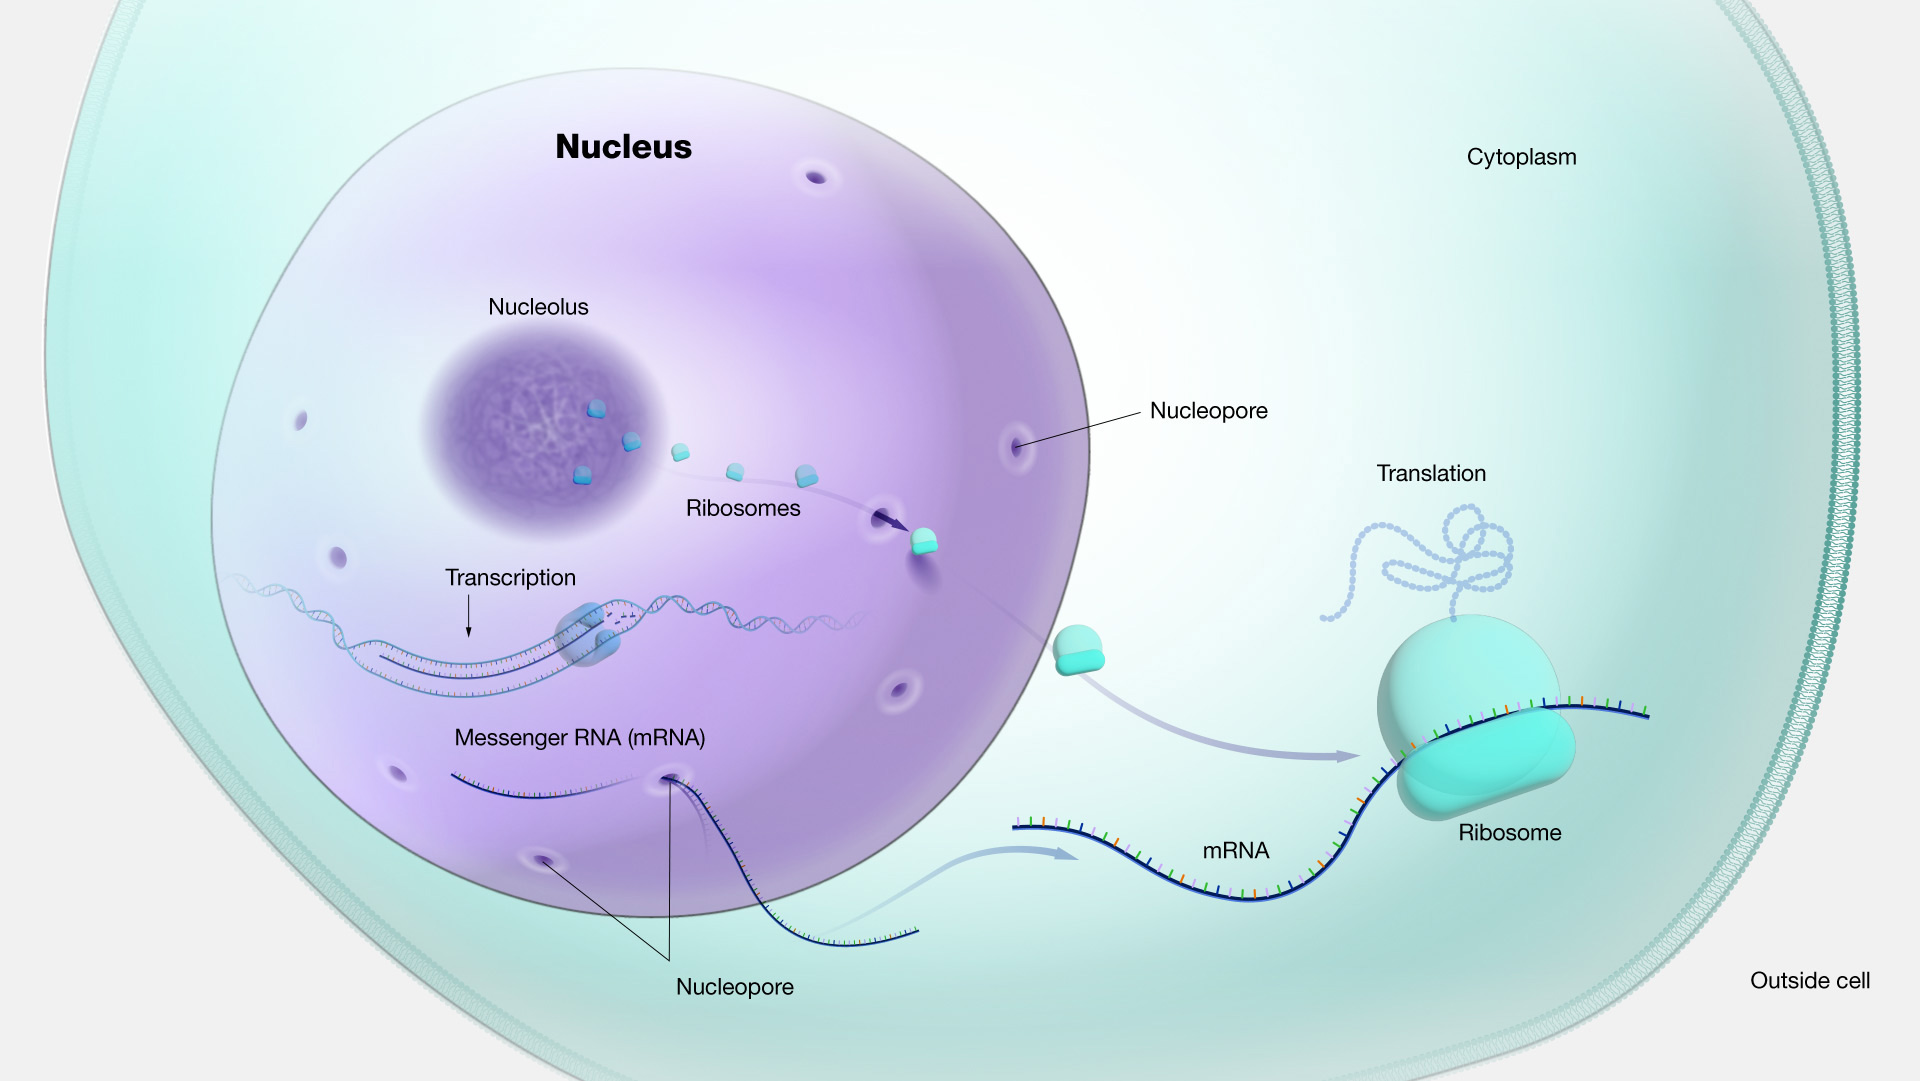
\includegraphics[width=\linewidth,height=5.3cm,keepaspectratio]{images/nucleus.jpg}
\par\smallskip{\fontsize{7}{9}\selectfont\color{NoteGray} 典型有核细胞的局部示意；颜色与大小用于说明结构，并非显微照片。\par}
\end{column}\begin{column}{.29\textwidth}\small
{\color{AcademicBlue}\bfseries 细胞核（Nucleus）}\par\smallskip 先找到紫色的核区域：这里保存着大部分 DNA。\par\medskip
{\color{AcademicBlue}\bfseries 细胞质（Cytoplasm）}\par\smallskip 核外仍有许多分子活动；核糖体参与蛋白质合成。\par\medskip
{\color{AcademicBlue}\bfseries 先记住空间关系}\par\smallskip 细胞核位于细胞内部；细胞膜是细胞与外界的边界。\par\medskip\end{column}\end{columns}
\source{来源：\href{https://www.cancer.gov/publications/dictionaries/cancer-terms/def/organ}{\mbox{NCI：器官（cancer.gov）}}\hspace{1em}\allowbreak \href{https://www.genome.gov/genetics-glossary}{\mbox{NHGRI：基础术语（genome.gov）}}\par \href{https://www.genome.gov/genetics-glossary/Nucleus}{图片：NHGRI}；\href{https://www.genome.gov/about-nhgri/Policies-Guidance/Copyright}{Public domain}；原图等比缩放。}
\note{先让听众定位大紫色细胞核，再看外侧浅青色细胞质；不要将核膜误认成整个细胞的边界。图中转录、mRNA和核糖体先作为预告，后面再解释。补充细胞核并不是细胞里唯一含DNA的地方，真核细胞的线粒体也有自己的DNA。}
\end{frame}

% PAGE 10 / 组织中的细胞具有不同分工
\begin{frame}{组织中的细胞具有不同分工}\relax
\par\noindent{\small\setlength{\tabcolsep}{7pt}\renewcommand{\arraystretch}{1.3}
\begin{tabularx}{\dimexpr\linewidth-4pt\relax}{@{}YYY@{}}\toprule
细胞类别 & 入门理解 & 在组织中的作用线索\\\midrule
上皮细胞 & 构成身体表面或器官内壁等结构 & 覆盖、屏障与相关组织结构\\
免疫细胞 & 参与机体防御 & 免疫反应与局部环境\\
成纤维细胞 & 参与支撑与修复 & 组织支持及修复过程\\
\bottomrule\end{tabularx}\par}

\source{依据：配套讲义第1章。}
\note{这三个名字是帮助建立初始直觉，不是完整的细胞分类。回到肿瘤切片，强调同一组织区域可以混合多种细胞，后面一个spot的信号也可能由它们共同贡献。}
\end{frame}

% PAGE 11 / 形态信息与分子信息
\begin{frame}{形态信息与分子信息}\relax
\begin{itemize}\wideitems
\item 显微图像提供细胞外形、排列和组织结构线索。
\item 专家可以依据形态作出许多判断。
\item 分子测量补充细胞身份、增殖或刺激响应等方面的线索。
\end{itemize}\keypoint{与贯穿案例的联系}{我们既想看见组织布局，也想识别其中的免疫相关细胞。}
\source{依据：配套讲义第1章。}
\note{不要把图像描述为没有价值。正确关系是形态和分子信息提供不同观察层次。下一步进入细胞内部，解释分子信号为什么可能反映身份与状态。}
\end{frame}

% PAGE 12 / 看真实组织图：形态能告诉我们什么？
\begin{frame}{看真实组织图：形态能告诉我们什么？}\relax
\begin{columns}[c,onlytextwidth]
\begin{column}{.43\textwidth}\centering
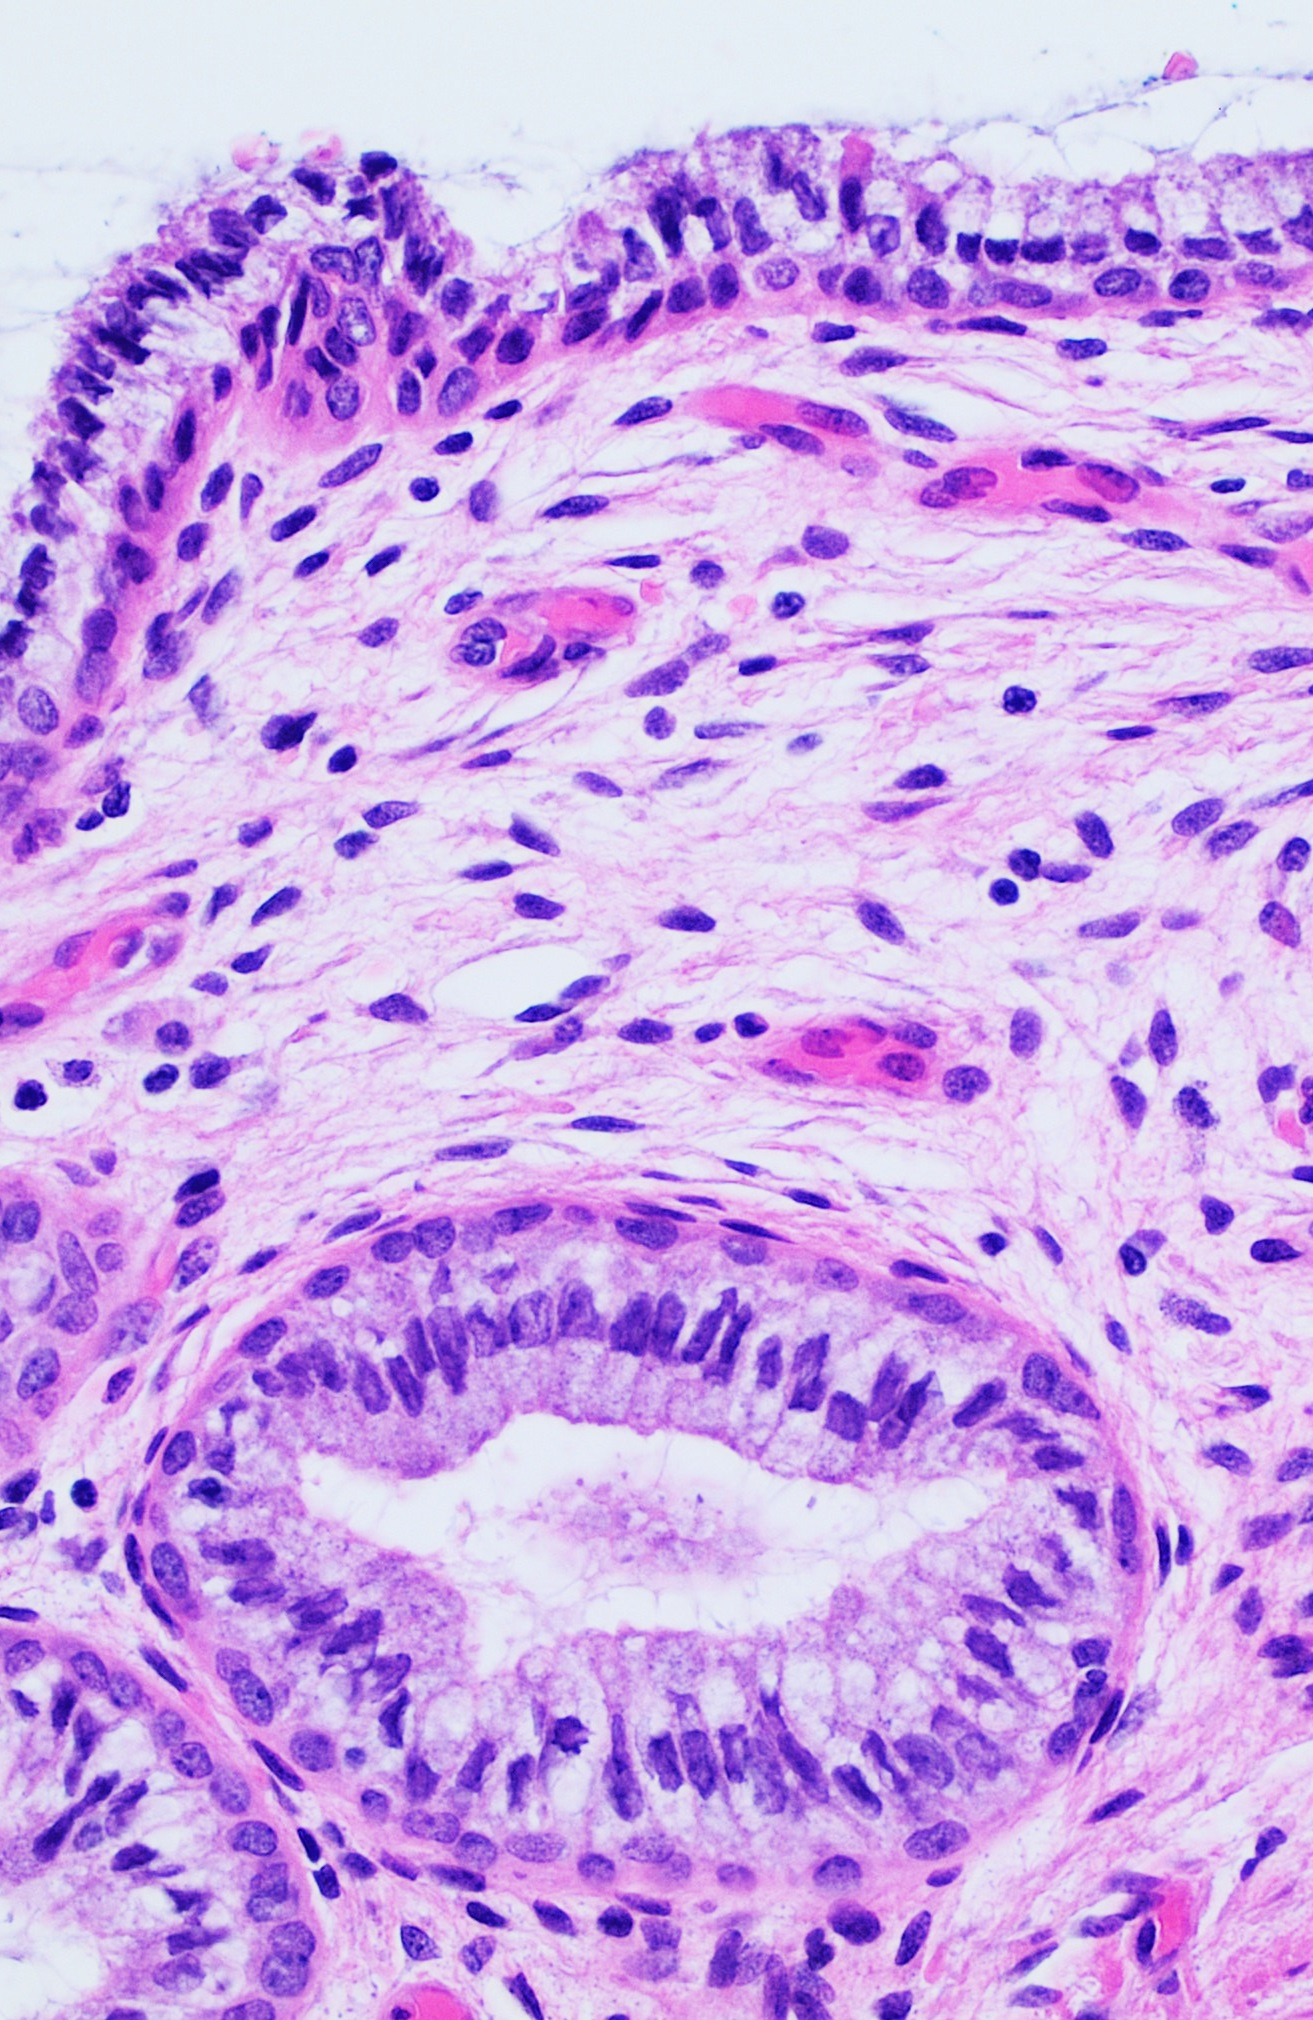
\includegraphics[width=\linewidth,height=5.45cm,keepaspectratio]{images/histology.jpg}
\par\smallskip{\fontsize{7}{9}\selectfont\color{NoteGray} 真实组织学图像；仅用于理解形态，不作为本汇报肿瘤案例的数据。\par}
\end{column}\begin{column}{.53\textwidth}\small
{\color{AcademicBlue}\bfseries 这是一张真实显微照片}\par\smallskip 宫颈管组织，采用苏木精—伊红（H\&E）染色。\par\medskip
{\color{AcademicBlue}\bfseries 先观察“如何排列”}\par\smallskip 比较深紫色核区域、表面上皮与下方腺体的组织方式。\par\medskip
{\color{AcademicBlue}\bfseries 再提出分子问题}\par\smallskip 哪些基因在这些位置表达？需要额外的分子测量来回答。\par\medskip\end{column}\end{columns}
\source{依据：配套讲义第1章。\par \href{https://commons.wikimedia.org/wiki/File:Histology_of_endocervix.jpg}{图片：Mikael H\"aggstr\"om}；\href{https://creativecommons.org/publicdomain/zero/1.0/}{CC0 1.0}；原图等比缩放。}
\note{说明这是来自独立公开来源的宫颈管组织学图像，不是贯穿全篇肿瘤案例的真实样本。H&E常让细胞核呈蓝紫色、其他结构呈不同粉色调。引导听众观察形态和排列，不要求做病理诊断，也不能用此染色直接读取RNA表达。}
\end{frame}

\subsection{第2章：DNA和基因}

% PAGE 13 / 第2章：DNA和基因
\begin{frame}{第2章：DNA和基因}\relax
\vfill\begin{center}\begin{minipage}{.86\linewidth}
{\large\color{AcademicBlue}本章导读\par}\vspace{4mm}
{\Large 本章区分 DNA、基因、染色体与基因组，说明遗传信息如何保存和组织。\par\vspace{4mm}随后我们将沿着这些信息，理解 RNA 的产生。\par}
\end{minipage}\end{center}\vfill
\source{依据：配套讲义第2章。}
\note{章节导入。本章区分 DNA、基因、染色体与基因组，说明遗传信息如何保存和组织。随后我们将沿着这些信息，理解 RNA 的产生。}
\end{frame}

% PAGE 14 / DNA：保存遗传信息的分子
\begin{frame}{DNA：保存遗传信息的分子}\relax
\begin{itemize}\wideitems
\item DNA是实际存在的分子，常以双螺旋结构表示。
\item A、T、C、G代表不同碱基，排列承载遗传信息。
\item 对CS读者，序列可以先表示为很长的字符串。
\end{itemize}\keypoint{字符串表示的边界}{真实DNA还涉及分子结构、包装与细胞环境。}
\source{来源：\href{https://www.genome.gov/genetics-glossary/Deoxyribonucleic-Acid-DNA}{\mbox{NHGRI：DNA（genome.gov）}}}
\note{用字符串类比建立熟悉感，再说明字符串不是生物分子的全部。这里关注保存的信息，为下一页区分DNA与基因做好准备。}
\end{frame}

% PAGE 15 / 看图理解 DNA：结构与序列是两个视角
\begin{frame}{看图理解 DNA：结构与序列是两个视角}\relax
\begin{columns}[c,onlytextwidth]
\begin{column}{.68\textwidth}\centering
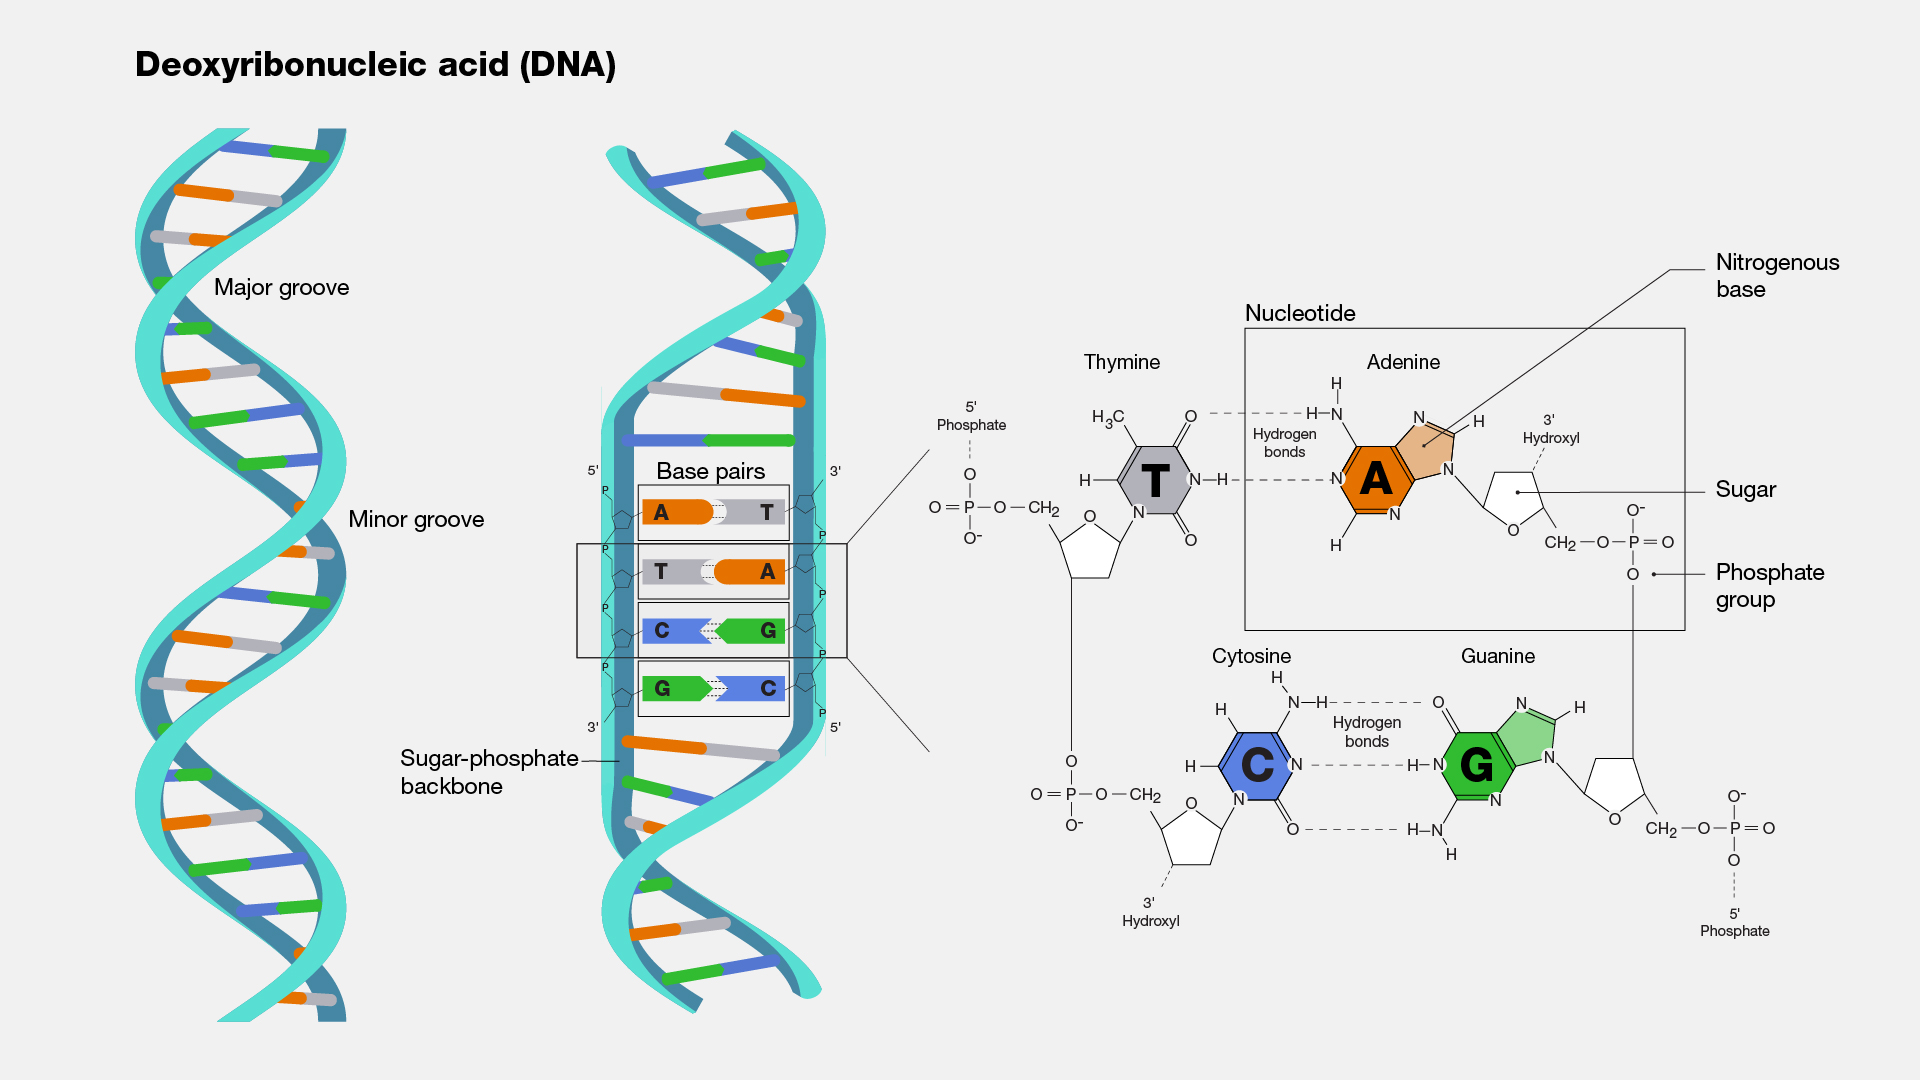
\includegraphics[width=\linewidth,height=5.3cm,keepaspectratio]{images/dna.jpg}
\par\smallskip{\fontsize{7}{9}\selectfont\color{NoteGray} DNA 结构示意；右侧化学细节用于定位概念，无须记忆。\par}
\end{column}\begin{column}{.29\textwidth}\small
{\color{AcademicBlue}\bfseries 看整体}\par\smallskip 左侧的两条链共同形成双螺旋。\par\medskip
{\color{AcademicBlue}\bfseries 看局部}\par\smallskip 中间放大了碱基配对：A 与 T、C 与 G。\par\medskip
{\color{AcademicBlue}\bfseries 回到数据}\par\smallskip 序列记录字母顺序；图像帮助理解分子的空间结构。\par\medskip\end{column}\end{columns}
\source{来源：\href{https://www.genome.gov/genetics-glossary/Deoxyribonucleic-Acid-DNA}{\mbox{NHGRI：DNA（genome.gov）}}\par \href{https://www.genome.gov/genetics-glossary/Deoxyribonucleic-Acid-DNA}{图片：NHGRI}；\href{https://www.genome.gov/about-nhgri/Policies-Guidance/Copyright}{Public domain}；原图等比缩放。}
\note{沿着左侧双螺旋到中间配对再到右侧化学结构讲解。面向CS和AI背景，只要求记住DNA既是物理分子，也可以用符号序列表示；本页不要求背化学结构。DNA信息不等于某个时刻的表达量。}
\end{frame}

% PAGE 16 / 基因：DNA上的功能区段
\begin{frame}{基因：DNA上的功能区段}\relax
\begin{itemize}\wideitems
\item 一个基因对应DNA上的特定区段。
\item 基因信息可以用于产生RNA。
\item 许多基因与蛋白质制造有关，一些RNA产物本身具有功能。
\item DNA上也有参与调控等作用的区域。
\end{itemize}
\source{来源：\href{https://www.genome.gov/genetics-glossary}{\mbox{NHGRI：基础术语（genome.gov）}}}
\note{可以把DNA类比为一本长说明书，基因像其中有具体用途的内容。强调基因不是整条DNA的别名，也不能把所有DNA都等同于蛋白质制造说明。}
\end{frame}

% PAGE 17 / DNA、染色体与基因组
\begin{frame}{DNA、染色体与基因组}\relax
\par\noindent{\small\setlength{\tabcolsep}{7pt}\renewcommand{\arraystretch}{1.3}
\begin{tabularx}{\dimexpr\linewidth-4pt\relax}{@{}YYY@{}}\toprule
概念 & 理解重点 & 与表达的区别\\\midrule
DNA & 保存信息的分子 & 信息载体\\
基因 & DNA上的特定功能区段 & 区段存在不表示当前高表达\\
染色体 & DNA与蛋白质形成的组织结构 & DNA的一种组织与包装层次\\
基因组 & 一套遗传信息 & 描述保存的信息，而非此刻表达状态\\
\bottomrule\end{tabularx}\par}

\source{来源：\href{https://www.genome.gov/genetics-glossary/Deoxyribonucleic-Acid-DNA}{\mbox{NHGRI：DNA（genome.gov）}}\hspace{1em}\allowbreak \href{https://www.genome.gov/genetics-glossary}{\mbox{NHGRI：基础术语（genome.gov）}}}
\note{按分子、区段、包装、一套信息这几个层次讲清，不需要加入染色体数目等额外知识。帮助听众避免把“有这个基因”与“这个基因当前表达高”混为一谈。}
\end{frame}

% PAGE 18 / 看图理解：DNA 怎样组织成染色体
\begin{frame}{看图理解：DNA 怎样组织成染色体}\relax
\begin{columns}[c,onlytextwidth]
\begin{column}{.68\textwidth}\centering
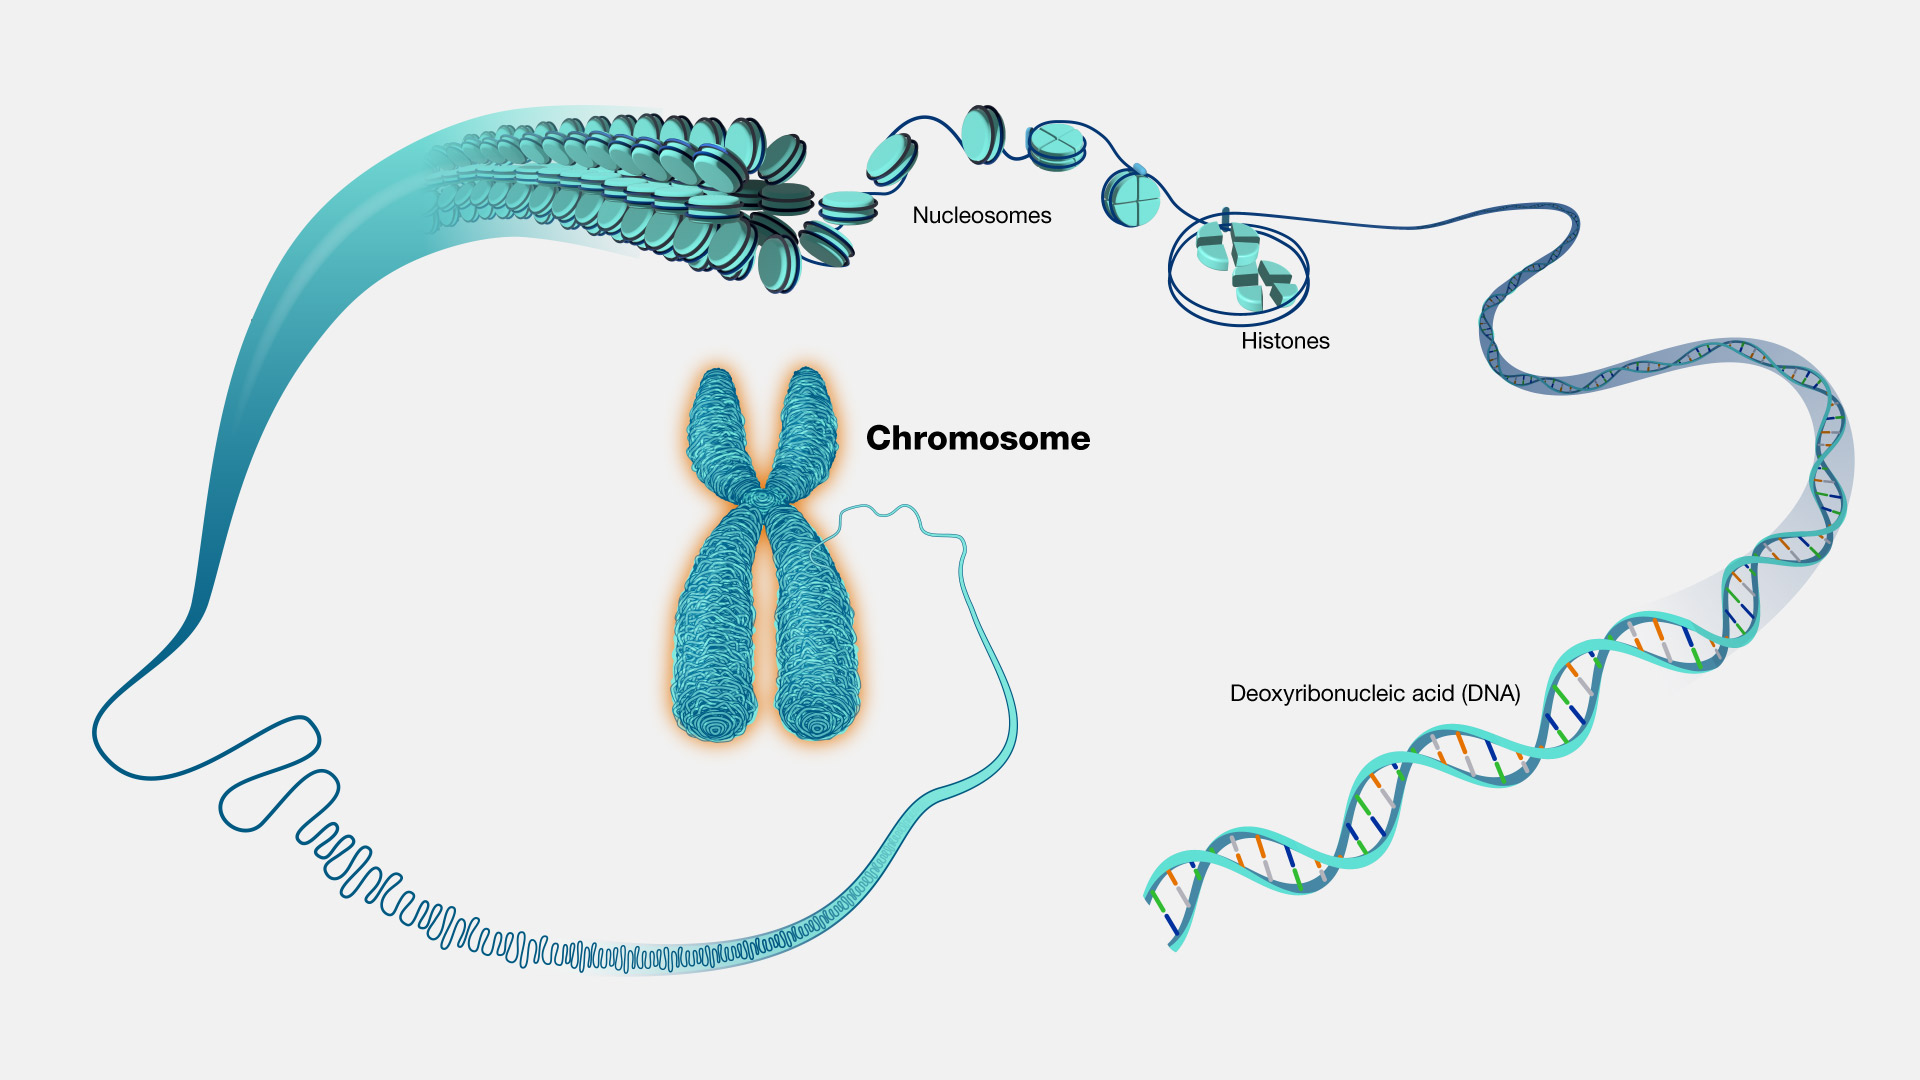
\includegraphics[width=\linewidth,height=5.3cm,keepaspectratio]{images/chromosome.jpg}
\par\smallskip{\fontsize{7}{9}\selectfont\color{NoteGray} 不同尺度的结构被放在同一图中；各部分不按统一比例绘制。\par}
\end{column}\begin{column}{.29\textwidth}\small
{\color{AcademicBlue}\bfseries 从右向左看}\par\smallskip DNA 双螺旋与蛋白质结合，并形成更高层次的包装结构。\par\medskip
{\color{AcademicBlue}\bfseries 区分两个概念}\par\smallskip 基因是 DNA 上的功能区段；染色体描述 DNA 的组织方式。\par\medskip
{\color{AcademicBlue}\bfseries 避免形状误解}\par\smallskip 图中的 X 形是特定阶段的示意，并非染色体一直呈 X 形。\par\medskip\end{column}\end{columns}
\source{来源：\href{https://www.genome.gov/genetics-glossary/Deoxyribonucleic-Acid-DNA}{\mbox{NHGRI：DNA（genome.gov）}}\hspace{1em}\allowbreak \href{https://www.genome.gov/genetics-glossary}{\mbox{NHGRI：基础术语（genome.gov）}}\par \href{https://www.genome.gov/genetics-glossary/Chromosome}{图片：NHGRI}；\href{https://www.genome.gov/about-nhgri/Policies-Guidance/Copyright}{Public domain}；原图等比缩放。}
\note{从右侧DNA开始追踪到缠绕结构和左侧更紧密的组织层次。这里的目的不是讲细胞分裂，而是把DNA、蛋白质和染色体这几个名词连起来。强调基因不是从DNA上分离出来的小颗粒；经典X形示意也不能当作所有阶段的染色体外形。}
\end{frame}

% PAGE 19 / 相似DNA与不同细胞功能
\begin{frame}{相似DNA与不同细胞功能}\relax
\begin{itemize}\wideitems
\item 同一个人的多数有核体细胞，基因组大体相同。
\item 神经细胞、免疫细胞等承担不同工作。
\item 重要原因之一：不同细胞使用的基因及使用程度不同。
\end{itemize}\keypoint{需要区分}{细胞保存了什么信息，与它现在如何使用信息，是两个问题。}
\source{来源：\href{https://www.genome.gov/genetics-glossary}{\mbox{NHGRI：基础术语（genome.gov）}}\hspace{1em}\allowbreak \href{https://www.genome.gov/genetics-glossary/Gene-Expression}{\mbox{NHGRI：基因表达（genome.gov）}}}
\note{不要说所有细胞的DNA完全相同，保留讲义中“大体相同”的范围。下一章从信息保存转向信息使用，解释转录怎样产生RNA。}
\end{frame}

\subsection{第3章：RNA和转录}

% PAGE 20 / 第3章：RNA和转录
\begin{frame}{第3章：RNA和转录}\relax
\vfill\begin{center}\begin{minipage}{.86\linewidth}
{\large\color{AcademicBlue}本章导读\par}\vspace{4mm}
{\Large 本章解释转录如何产生 RNA，并区分 RNA、mRNA 与转录本。\par\vspace{4mm}理解这一过程，才能读懂后面“测 RNA”究竟在测什么。\par}
\end{minipage}\end{center}\vfill
\source{依据：配套讲义第3章。}
\note{章节导入。本章解释转录如何产生 RNA，并区分 RNA、mRNA 与转录本。理解这一过程，才能读懂后面“测 RNA”究竟在测什么。}
\end{frame}

% PAGE 21 / 转录：根据DNA信息产生RNA
\begin{frame}{转录：根据DNA信息产生RNA}\relax
\begin{itemize}\wideitems
\item RNA是另一类实际存在的分子。
\item 细胞按照DNA中的相应信息合成RNA，称为转录。
\item 同一段基因信息可以对应多个RNA分子。
\end{itemize}\keypoint{说明书与工作副本的类比}{RNA可以像当前工作所需的副本，DNA原有信息仍然保留。}
\source{来源：\href{https://www.genome.gov/genetics-glossary/Transcription}{\mbox{NHGRI：转录（genome.gov）}}}
\note{类比只用于说明信息关系，不表示DNA和RNA化学组成完全相同。明确转录不是把整条DNA变成RNA，也不消耗掉原来的DNA。}
\end{frame}

% PAGE 22 / 看图理解转录：从 DNA 到 RNA
\begin{frame}{看图理解转录：从 DNA 到 RNA}\relax
\begin{columns}[c,onlytextwidth]
\begin{column}{.68\textwidth}\centering
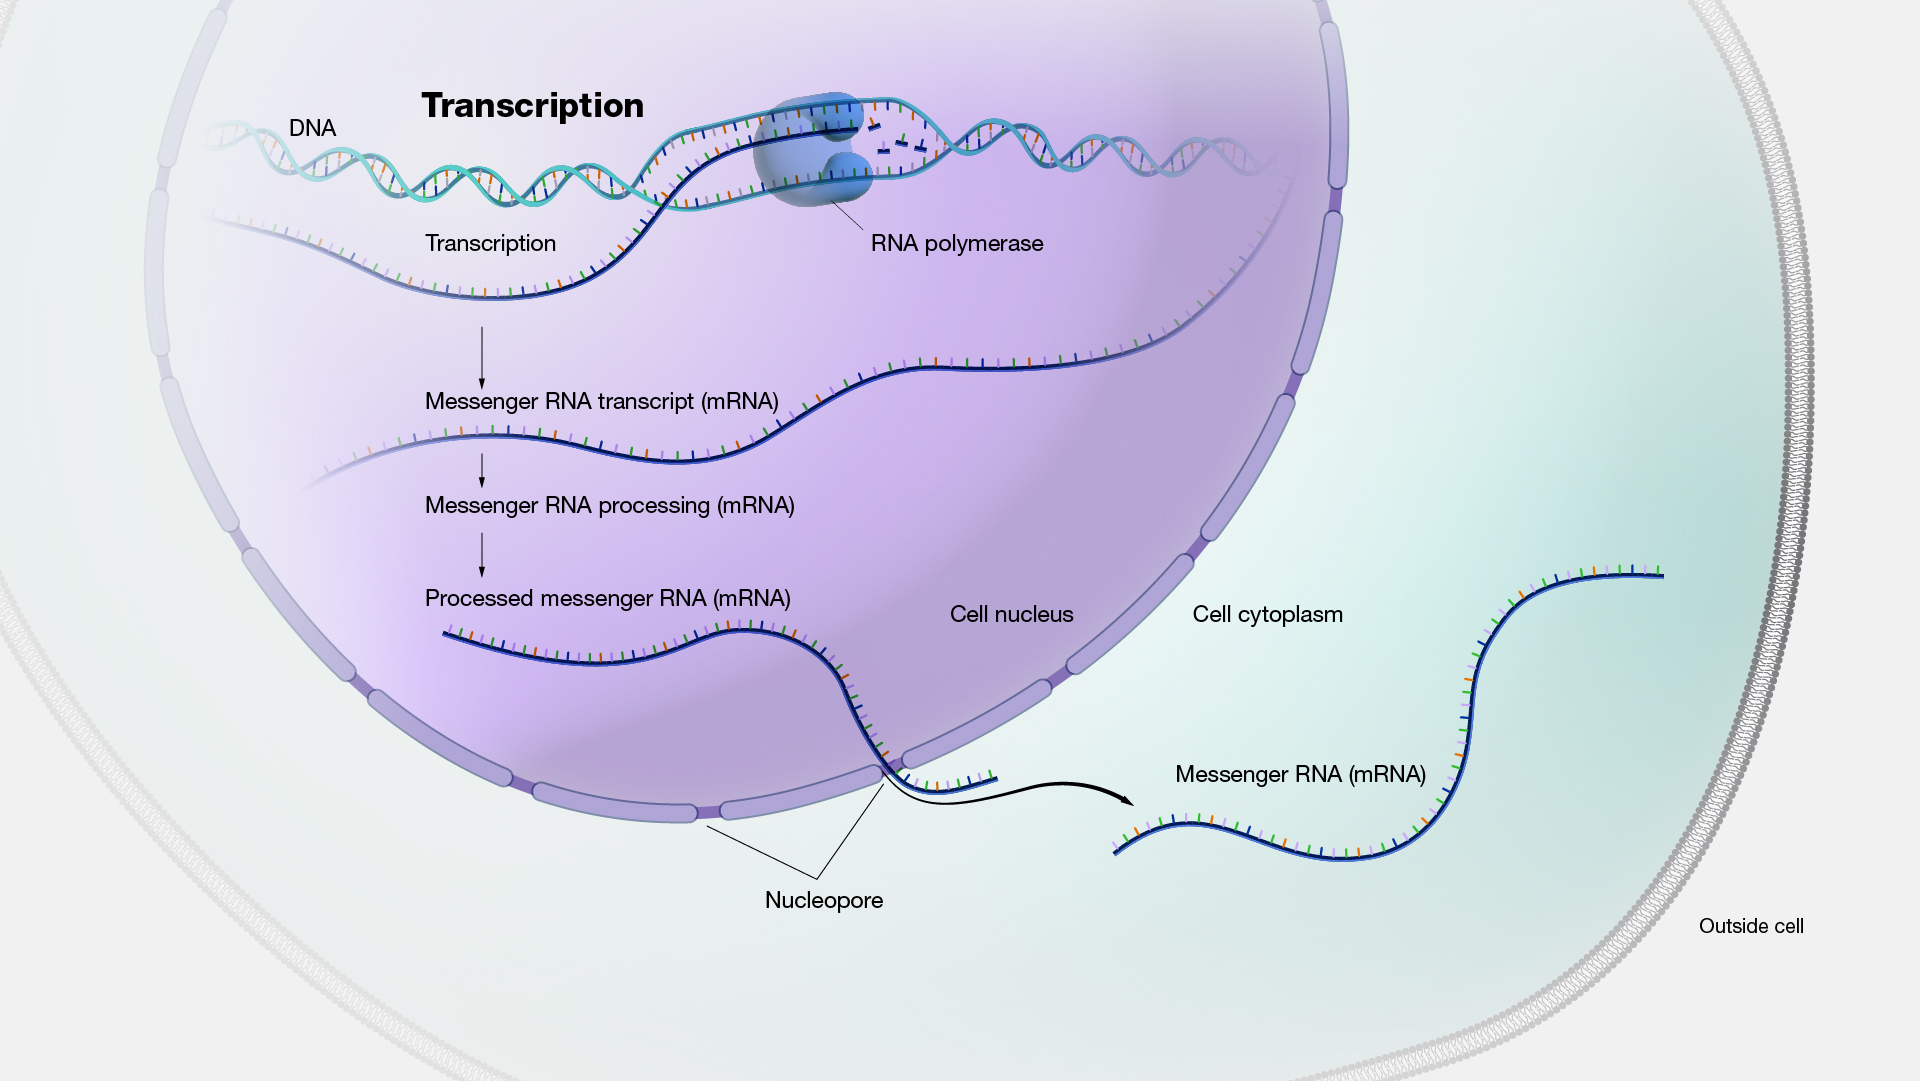
\includegraphics[width=\linewidth,height=5.3cm,keepaspectratio]{images/transcription.jpg}
\par\smallskip{\fontsize{7}{9}\selectfont\color{NoteGray} 真核细胞中的转录与 mRNA 加工示意；并非所有 RNA 都进入翻译。\par}
\end{column}\begin{column}{.29\textwidth}\small
{\color{AcademicBlue}\bfseries 第一步：产生 RNA}\par\smallskip RNA 聚合酶（RNA polymerase）根据 DNA 模板合成 RNA。\par\medskip
{\color{AcademicBlue}\bfseries 第二步：加工与输出}\par\smallskip 图示真核细胞中，mRNA 经加工后可离开细胞核。\par\medskip
{\color{AcademicBlue}\bfseries 抓住主线}\par\smallskip 本页先看“产生 RNA”；蛋白质合成放在后面解释。\par\medskip\end{column}\end{columns}
\source{来源：\href{https://www.genome.gov/genetics-glossary/Transcription}{\mbox{NHGRI：转录（genome.gov）}}\par \href{https://www.genome.gov/genetics-glossary/Transcription}{图片：NHGRI}；\href{https://www.genome.gov/about-nhgri/Policies-Guidance/Copyright}{Public domain}；原图等比缩放。}
\note{先指出顶部转录区域，再沿RNA到下方成熟mRNA和核孔。图中画出了RNA加工，但初学者不必此时记住每一步。明确RNA加工不同于翻译；图是典型真核细胞的mRNA路线，不代表所有RNA都离核或都能编码蛋白质。}
\end{frame}

% PAGE 23 / RNA与mRNA的包含关系
\begin{frame}{RNA与mRNA的包含关系}\relax
\begin{itemize}\wideitems
\item mRNA是信使RNA，携带用于制造蛋白质的信息。
\item mRNA只是RNA的一个子类。
\item 其他RNA可以参与蛋白质制造、调控或承担其他功能。
\end{itemize}\keypoint{后续路线}{mRNA可以进入翻译过程，部分其他RNA本身就是功能产物。}
\source{来源：\href{https://www.genome.gov/genetics-glossary/Messenger-RNA-mRNA}{\mbox{NHGRI：mRNA（genome.gov）}}}
\note{不要让听众形成所有RNA都会变成蛋白质的印象。这里先建立包含关系，不要求记住全部RNA类别。}
\end{frame}

% PAGE 24 / 看图理解：RNA 不只有 mRNA
\begin{frame}{看图理解：RNA 不只有 mRNA}\relax
\begin{columns}[c,onlytextwidth]
\begin{column}{.68\textwidth}\centering
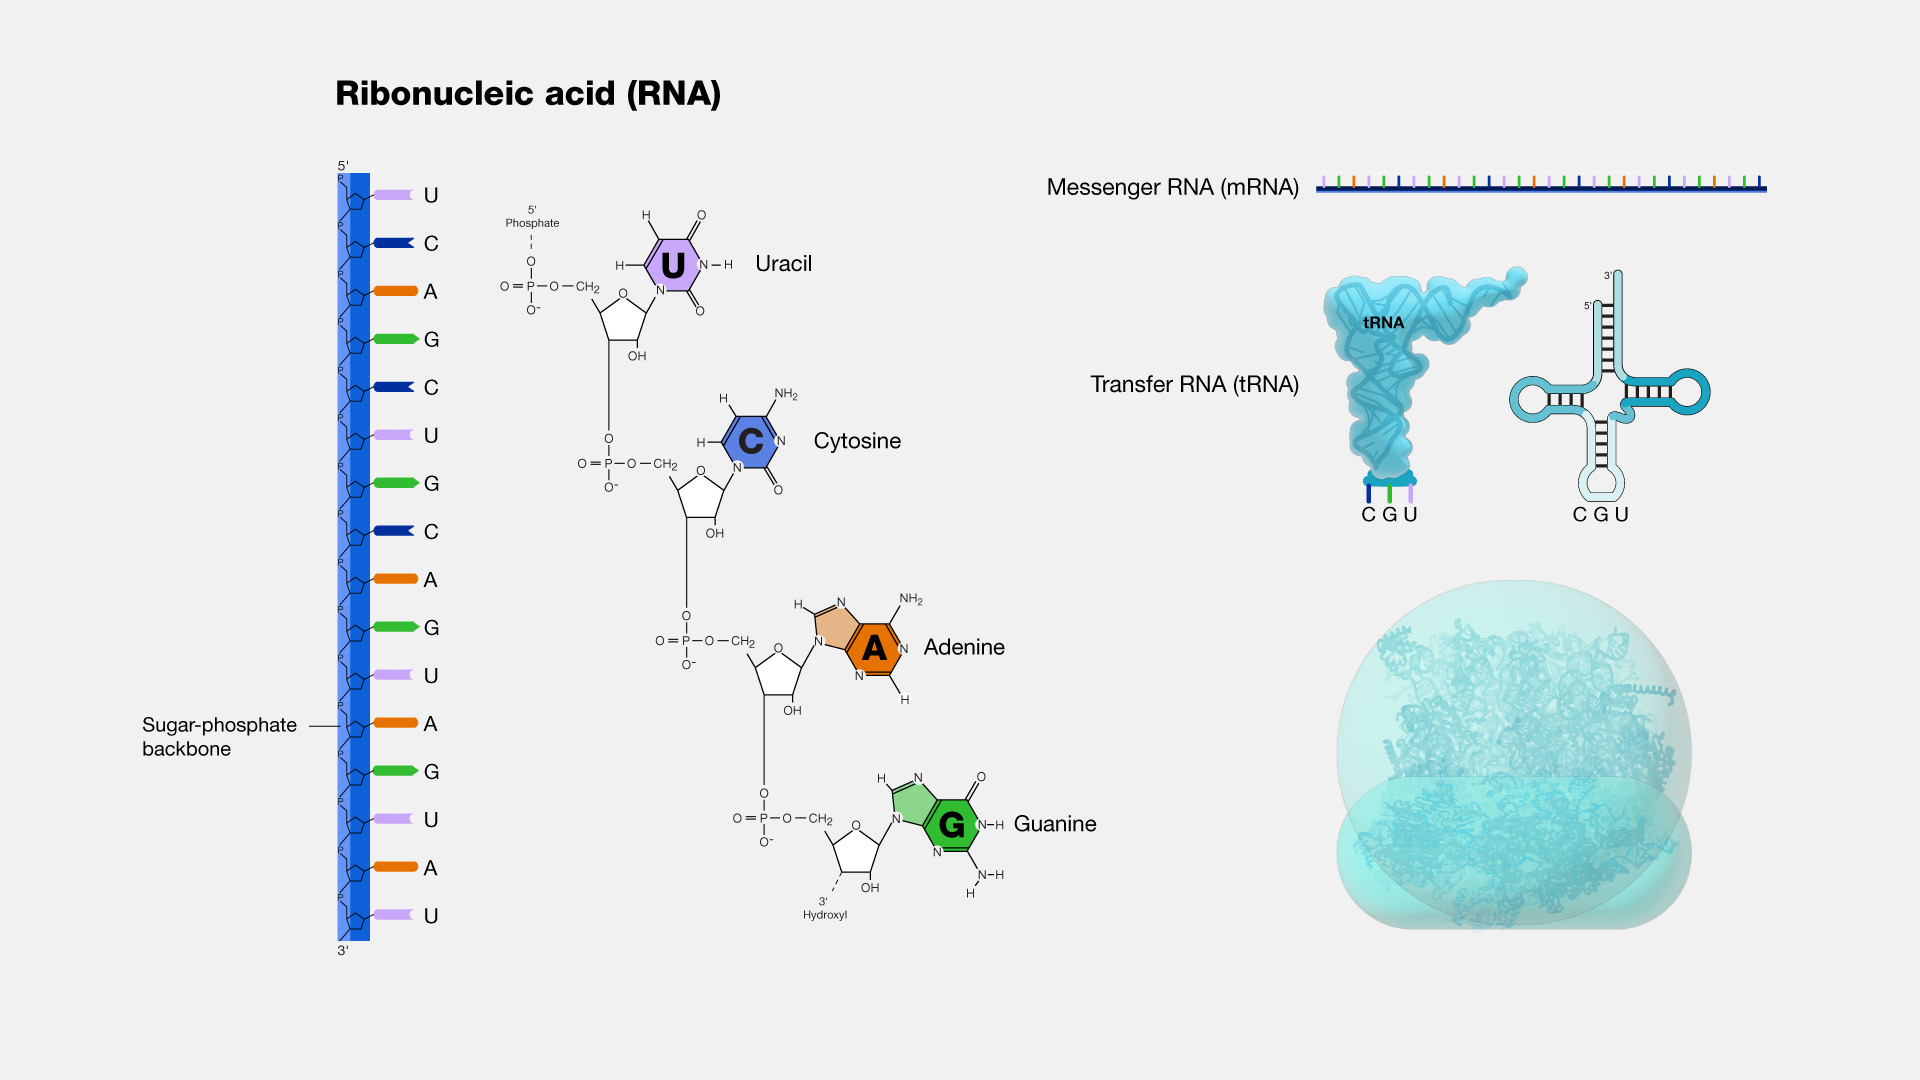
\includegraphics[width=\linewidth,height=5.3cm,keepaspectratio]{images/rna.jpg}
\par\smallskip{\fontsize{7}{9}\selectfont\color{NoteGray} RNA 类别与结构示意：左侧为局部结构，右侧为若干 RNA 类型。\par}
\end{column}\begin{column}{.29\textwidth}\small
{\color{AcademicBlue}\bfseries mRNA：传递编码信息}\par\smallskip 右上方示意可被翻译的信使 RNA。\par\medskip
{\color{AcademicBlue}\bfseries tRNA、rRNA：参与合成}\par\smallskip 转运 RNA 和核糖体 RNA 也参与蛋白质合成。\par\medskip
{\color{AcademicBlue}\bfseries 形态不止一条直线}\par\smallskip RNA 可以形成复杂结构；“RNA”不能直接替换为“mRNA”。\par\medskip\end{column}\end{columns}
\source{来源：\href{https://www.genome.gov/genetics-glossary/Messenger-RNA-mRNA}{\mbox{NHGRI：mRNA（genome.gov）}}\par \href{https://www.genome.gov/genetics-glossary/Ribonucleic-Acid-RNA}{图片：NHGRI}；\href{https://www.genome.gov/about-nhgri/Policies-Guidance/Copyright}{Public domain}；原图等比缩放。}
\note{将三种RNA的缩写与中文名称对应起来：mRNA信使RNA、tRNA转运RNA、rRNA核糖体RNA。只要求理解包含关系和大致角色。不同空间转录组实验所富集或检测的RNA范围取决于技术，不能看到RNA两个字就默认所有类型都同样被测到。}
\end{frame}

% PAGE 25 / RNA组合提供身份与状态线索
\begin{frame}{RNA组合提供身份与状态线索}\relax
\begin{itemize}\wideitems
\item 不同细胞可以呈现不同的RNA组合。
\item 同一种细胞在受到刺激后，RNA组合也可能变化。
\item 研究人员依据多种表达信号，分析细胞身份与当前状态。
\end{itemize}
\source{来源：\href{https://www.genome.gov/genetics-glossary/Gene-Expression}{\mbox{NHGRI：基因表达（genome.gov）}}\hspace{1em}\allowbreak \href{https://www.genome.gov/about-genomics/fact-sheets/Transcriptome-Fact-Sheet}{\mbox{NHGRI：转录组（genome.gov）}}}
\note{回到肿瘤薄片：免疫相关表达组合可以提示某些位置值得进一步检查，但并不是实验直接打印了一个“免疫细胞”标签。后续还需要注释或其他推断。}
\end{frame}

% PAGE 26 / RNA水平与产生速度
\begin{frame}{RNA水平与产生速度}\relax
\begin{itemize}\wideitems
\item 测得的RNA水平受合成与降解共同影响。
\item 捕获、测序或成像过程也影响最终记录到的信号。
\item 某类RNA较多，不能直接解释为此刻产生速度一定更快。
\end{itemize}\keypoint{我们分析的起点}{实验记录到的RNA信号，以及它与真实生物过程之间的联系。}
\source{依据：配套讲义第3章。}
\note{可以用水池中的水量类比库存，但说明本页没有建立具体动力学模型。重点是让听众把“测量值”与“想解释的过程”分开。}
\end{frame}

\subsection{第4章：蛋白质与翻译}

% PAGE 27 / 第4章：蛋白质与翻译
\begin{frame}{第4章：蛋白质与翻译}\relax
\vfill\begin{center}\begin{minipage}{.86\linewidth}
{\large\color{AcademicBlue}本章导读\par}\vspace{4mm}
{\Large 本章介绍翻译、蛋白质结构及其功能，串起从 DNA 到 RNA 再到蛋白质的关系。\par\vspace{4mm}由此理解，RNA 信号与蛋白质含量、功能之间仍有需要验证的环节。\par}
\end{minipage}\end{center}\vfill
\source{依据：配套讲义第4章。}
\note{章节导入。本章介绍翻译、蛋白质结构及其功能，串起从 DNA 到 RNA 再到蛋白质的关系。由此理解，RNA 信号与蛋白质含量、功能之间仍有需要验证的环节。}
\end{frame}

% PAGE 28 / 蛋白质：由氨基酸链形成的分子
\begin{frame}{蛋白质：由氨基酸链形成的分子}\relax
\begin{itemize}\wideitems
\item 蛋白质通常由一条或多条氨基酸链构成。
\item 氨基酸按一定顺序连接，链再折叠成结构。
\item 序列影响结构，结构与功能密切相关。
\end{itemize}
\source{来源：\href{https://www.genome.gov/genetics-glossary/Protein}{\mbox{NHGRI：蛋白质（genome.gov）}}}
\note{可以用不同珠子串成链再折叠的类比。强调蛋白质是具体分子，不是抽象的功能标签。}
\end{frame}

% PAGE 29 / 看图理解蛋白质：从链到空间结构
\begin{frame}{看图理解蛋白质：从链到空间结构}\relax
\begin{columns}[c,onlytextwidth]
\begin{column}{.68\textwidth}\centering
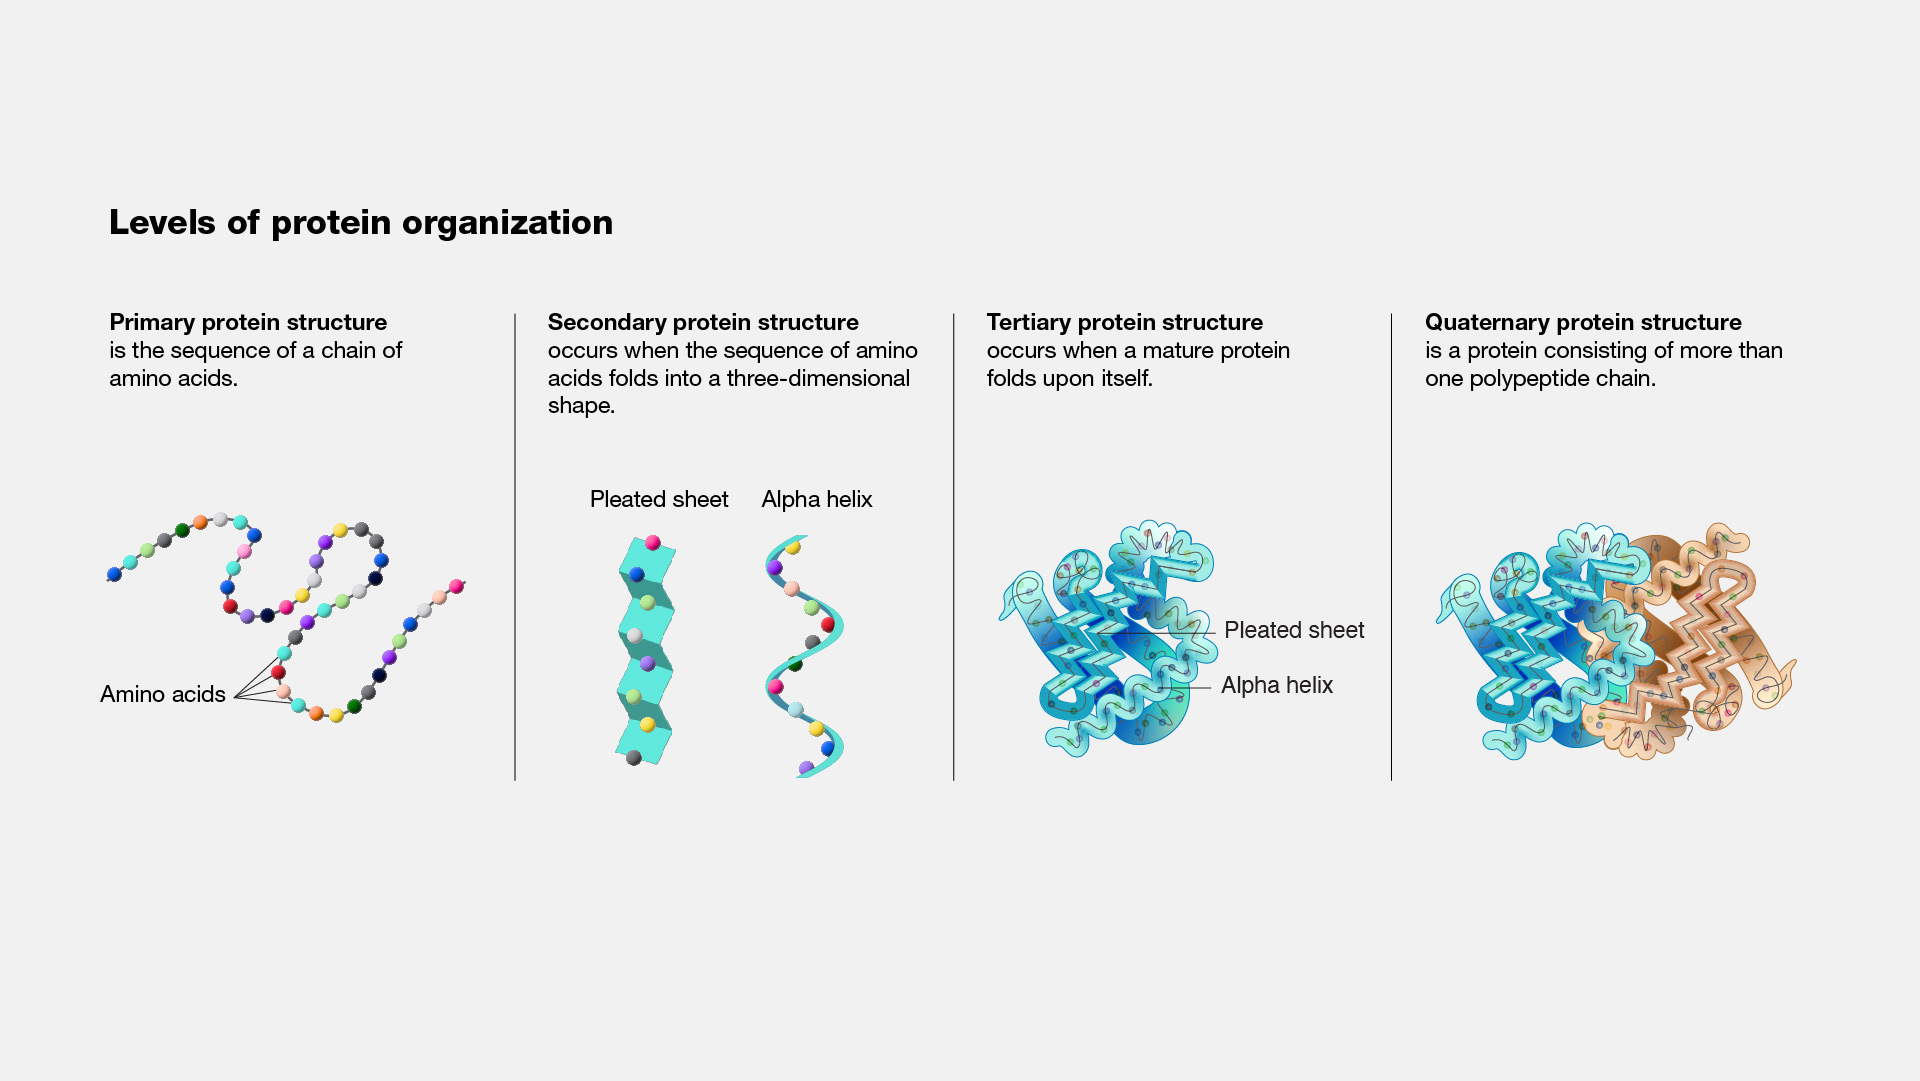
\includegraphics[width=\linewidth,height=5.3cm,keepaspectratio]{images/protein.jpg}
\par\smallskip{\fontsize{7}{9}\selectfont\color{NoteGray} 从左到右：序列、局部结构、整体折叠、多链组装。\par}
\end{column}\begin{column}{.29\textwidth}\small
{\color{AcademicBlue}\bfseries 先看左侧的链}\par\smallskip 氨基酸按顺序连接，形成多肽链。\par\medskip
{\color{AcademicBlue}\bfseries 再看局部与整体}\par\smallskip 链可形成局部结构，并折叠成整体空间形状。\par\medskip
{\color{AcademicBlue}\bfseries 有些还会组装}\par\smallskip 多个链可组成复合体；不要求所有蛋白质都具有同样层次。\par\medskip\end{column}\end{columns}
\source{来源：\href{https://www.genome.gov/genetics-glossary/Protein}{\mbox{NHGRI：蛋白质（genome.gov）}}\par \href{https://www.genome.gov/genetics-glossary/Protein}{图片：NHGRI}；\href{https://www.genome.gov/about-nhgri/Policies-Guidance/Copyright}{Public domain}；原图等比缩放。}
\note{按四栏依次讲：一级结构是氨基酸顺序，二级结构是局部规律结构，三级结构是单条链整体构象，四级结构描述多链组装。此处不用听众背四个结构名称，只建立蛋白质是有空间结构的分子这一认识。并非每种蛋白都有四级结构。}
\end{frame}

% PAGE 30 / 翻译：根据mRNA制造蛋白质
\begin{frame}{翻译：根据mRNA制造蛋白质}\relax
\begin{itemize}\wideitems
\item 核糖体等分子机器读取mRNA的信息。
\item 氨基酸按相应顺序连接，形成蛋白质相关产物。
\item 分子生物学中的“翻译”与自然语言翻译是不同任务。
\end{itemize}\keypoint{与转录区分}{转录产生RNA；翻译利用mRNA的信息制造蛋白质。}
\source{来源：\href{https://www.genome.gov/genetics-glossary/Translation}{\mbox{NHGRI：翻译（genome.gov）}}}
\note{只讲清两步的输入和产物。这里不扩展密码子等细节，因为本汇报的目标是理解空间RNA测量，而不是完整分子生物学课程。}
\end{frame}

% PAGE 31 / 看图理解翻译：核糖体读取 mRNA
\begin{frame}{看图理解翻译：核糖体读取 mRNA}\relax
\begin{columns}[c,onlytextwidth]
\begin{column}{.68\textwidth}\centering
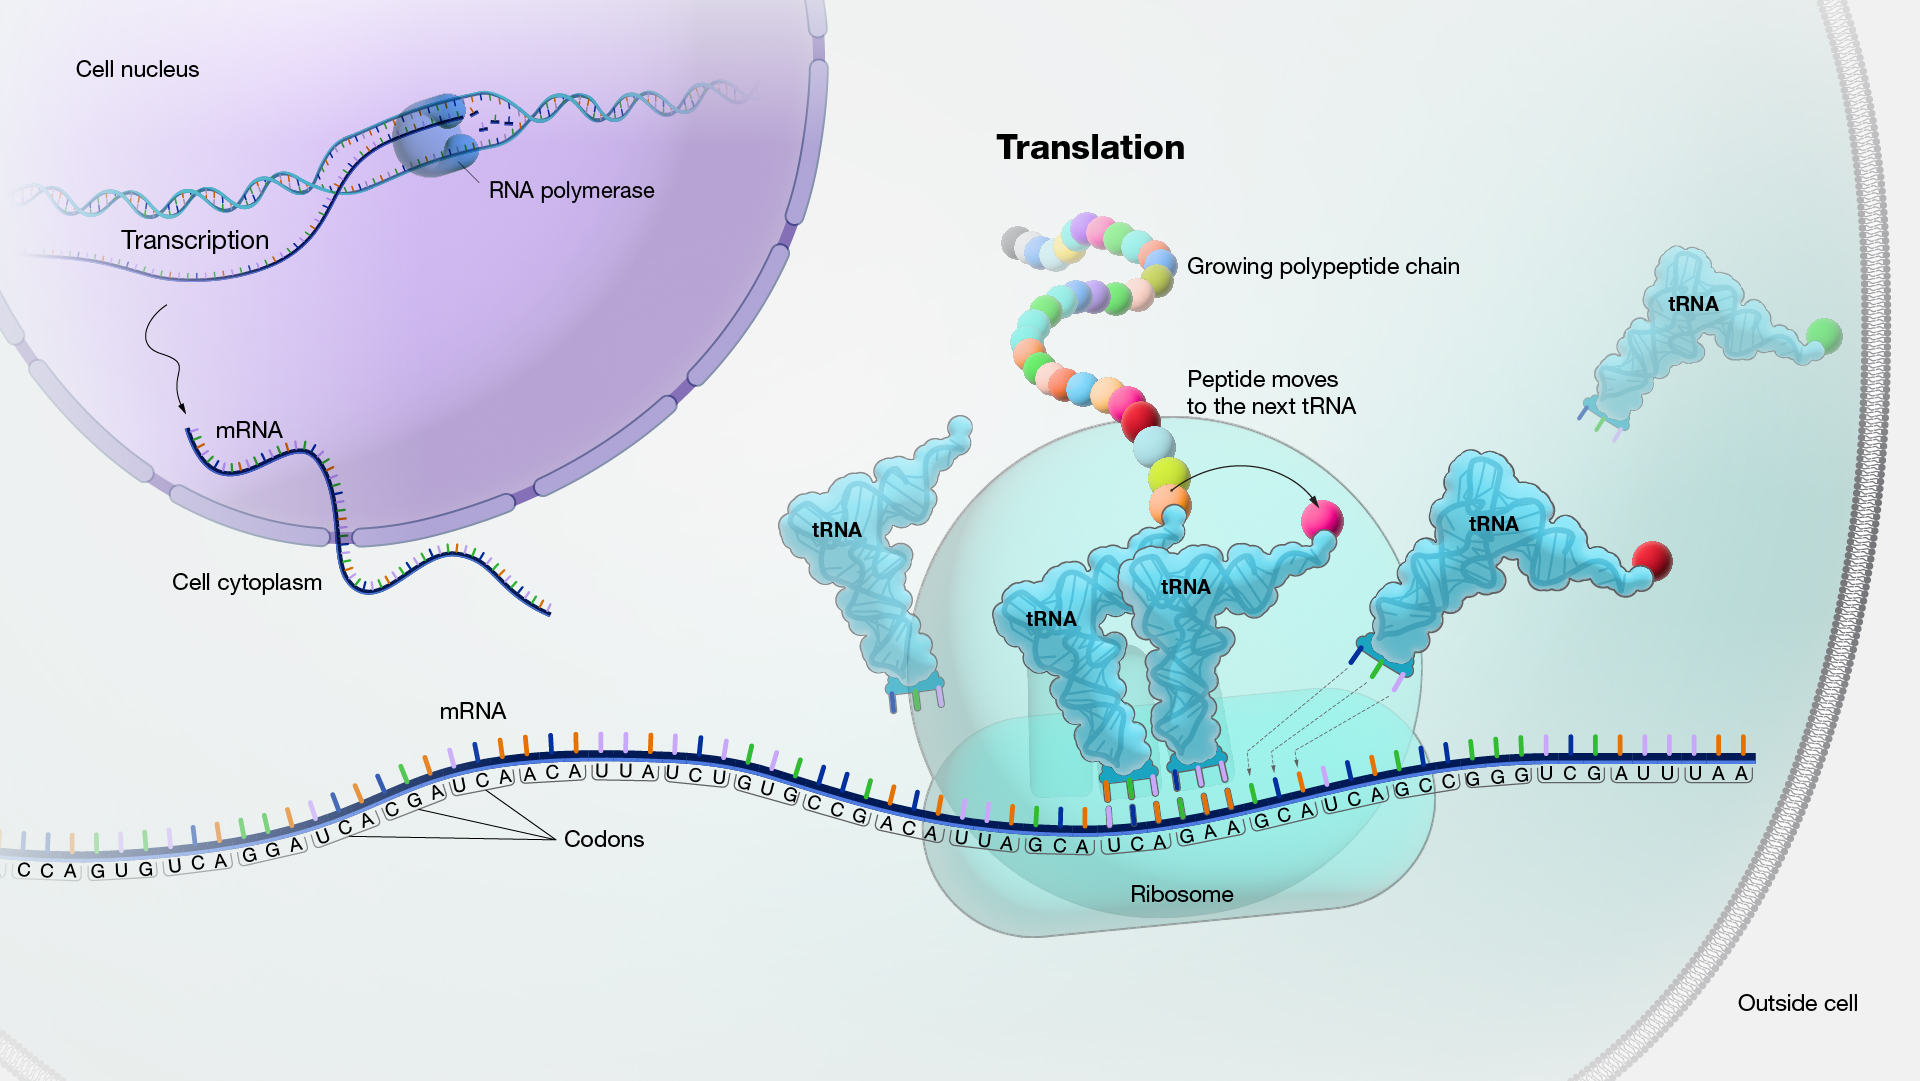
\includegraphics[width=\linewidth,height=5.3cm,keepaspectratio]{images/translation.jpg}
\par\smallskip{\fontsize{7}{9}\selectfont\color{NoteGray} 翻译过程示意；彩色小球与分子结构为教学表示。\par}
\end{column}\begin{column}{.29\textwidth}\small
{\color{AcademicBlue}\bfseries 找到 mRNA}\par\smallskip 下方的长链携带可读取的编码信息。\par\medskip
{\color{AcademicBlue}\bfseries 找到核糖体}\par\smallskip 蓝绿色结构与 mRNA 结合，参与合成多肽链。\par\medskip
{\color{AcademicBlue}\bfseries 观察正在延长的链}\par\smallskip 彩色小球串代表逐步连接的氨基酸；随后还可能折叠、加工。\par\medskip\end{column}\end{columns}
\source{来源：\href{https://www.genome.gov/genetics-glossary/Translation}{\mbox{NHGRI：翻译（genome.gov）}}\par \href{https://www.genome.gov/genetics-glossary/Translation}{图片：NHGRI}；\href{https://www.genome.gov/about-nhgri/Policies-Guidance/Copyright}{Public domain}；原图等比缩放。}
\note{让听众分别指认mRNA、核糖体和正在延长的多肽链。tRNA运送对应氨基酸，核糖体参与将其连接。强调蛋白质并不是RNA折叠变成的；RNA提供信息，氨基酸提供构建多肽链的原料。转录和翻译不要混淆。}
\end{frame}

% PAGE 32 / 蛋白质承担许多具体功能
\begin{frame}{蛋白质承担许多具体功能}\relax
\par\noindent{\small\setlength{\tabcolsep}{7pt}\renewcommand{\arraystretch}{1.3}
\begin{tabularx}{\dimexpr\linewidth-4pt\relax}{@{}YY@{}}\toprule
例子 & 功能线索\\\midrule
酶 & 帮助化学反应进行\\
血红蛋白 & 运输氧气\\
抗体 & 参与防御\\
受体 & 接收相关分子信号\\
\bottomrule\end{tabularx}\par}

\source{来源：\href{https://www.genome.gov/genetics-glossary/Protein}{\mbox{NHGRI：蛋白质（genome.gov）}}}
\note{补充单个蛋白质处在分子尺度，但大量蛋白质组成的材料可以看见，如头发和肌肉。蛋清含蛋白质也含大量水，避免把材料与纯蛋白混淆。}
\end{frame}

% PAGE 33 / 一个具体例子：血红蛋白的结构模型
\begin{frame}{一个具体例子：血红蛋白的结构模型}\relax
\begin{columns}[c,onlytextwidth]
\begin{column}{.46\textwidth}\centering
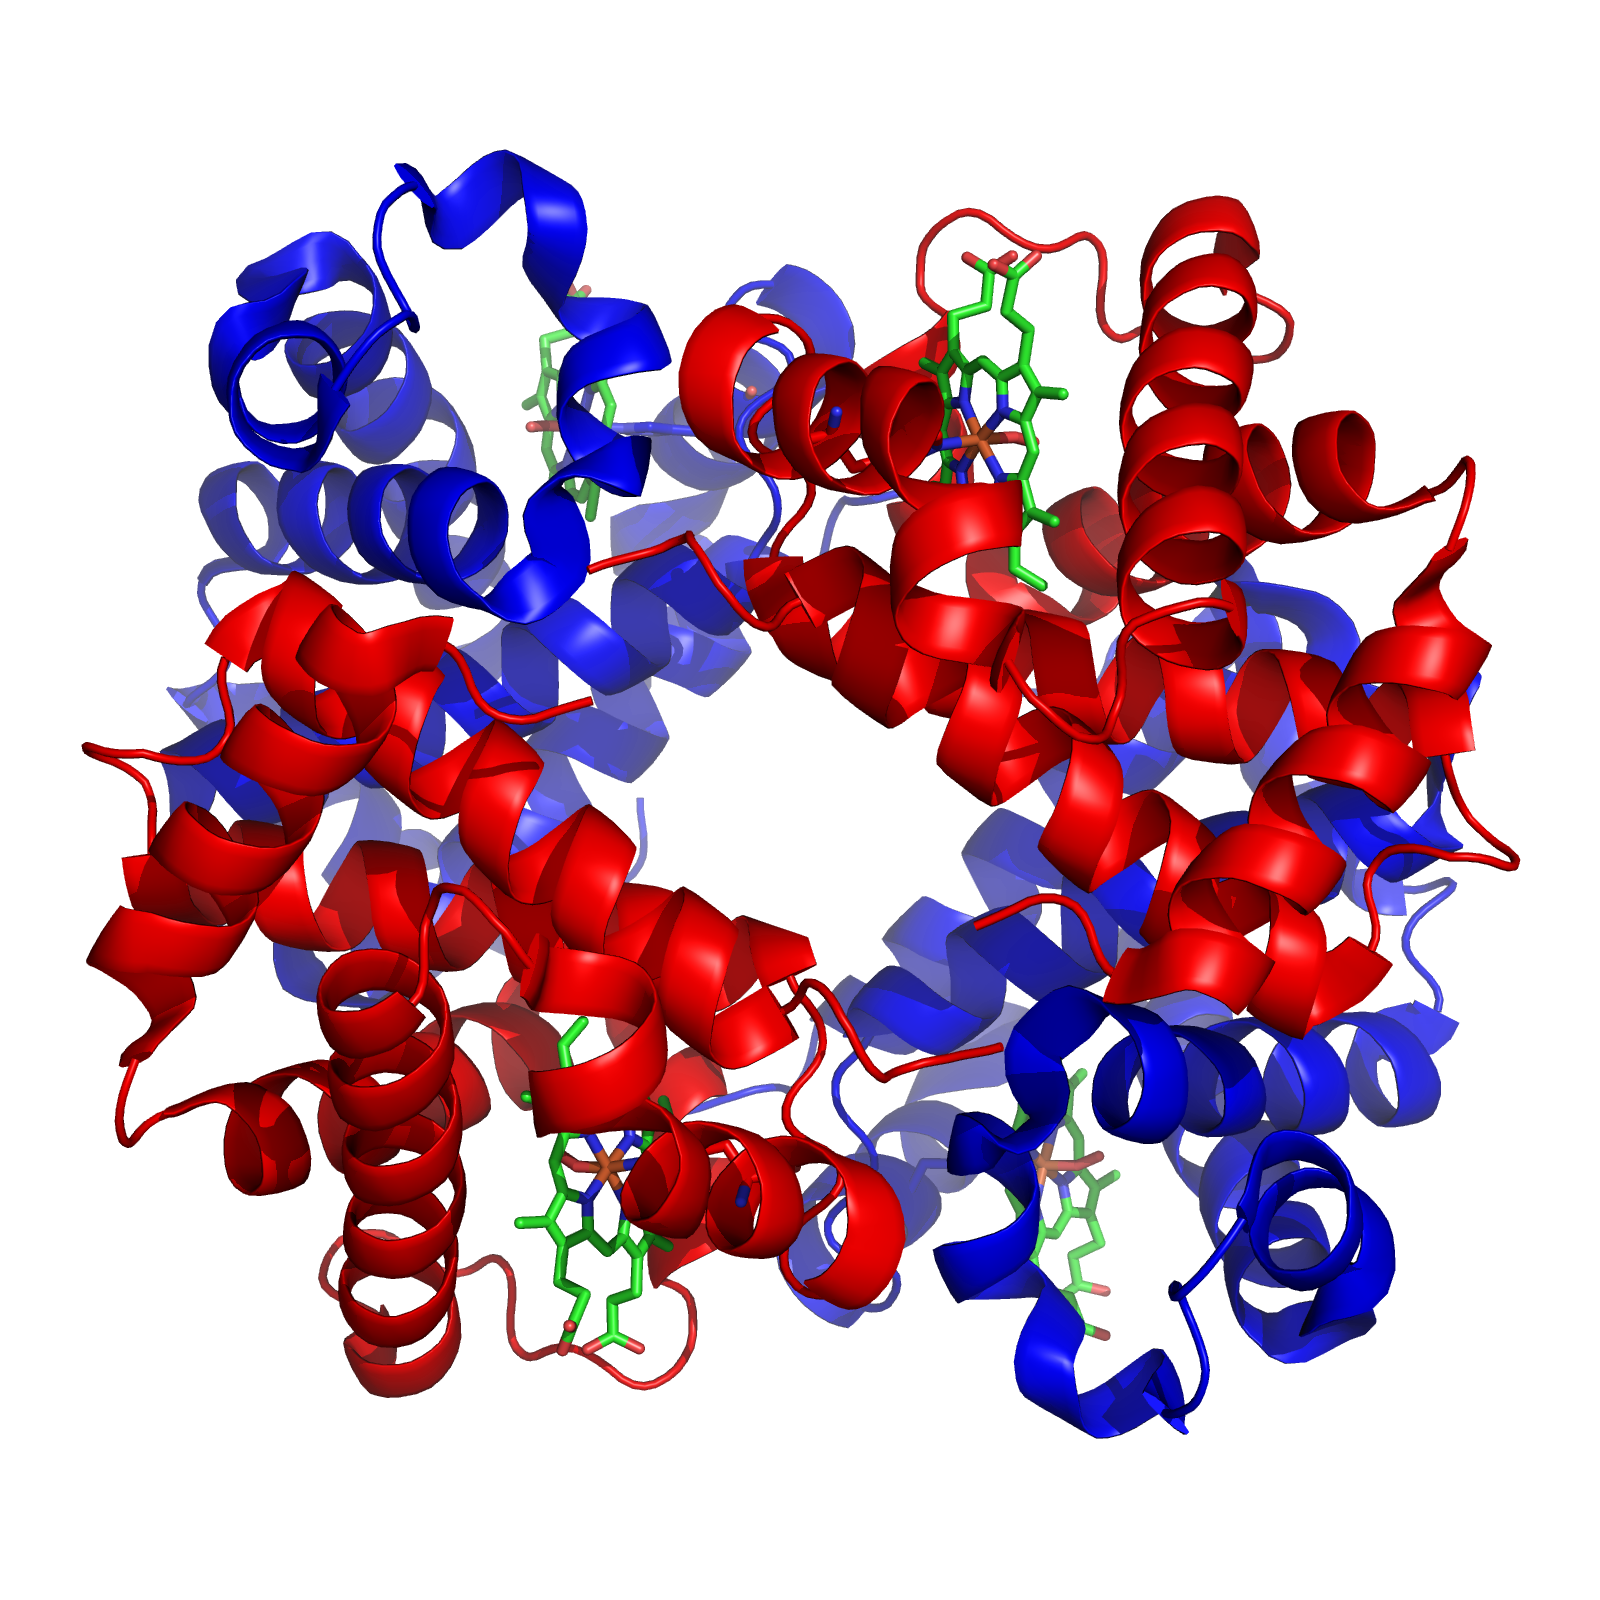
\includegraphics[width=\linewidth,height=5.1cm,keepaspectratio]{images/hemoglobin.png}
\par\smallskip{\fontsize{7}{9}\selectfont\color{NoteGray} 结构模型，非显微照片；保留原图，不把绘图颜色当成真实分子颜色。\par}
\end{column}\begin{column}{.50\textwidth}\small
{\color{AcademicBlue}\bfseries 这张图展示什么？}\par\smallskip 根据 PDB 1GZX 绘制的血红蛋白三维结构模型。\par\medskip
{\color{AcademicBlue}\bfseries 怎样读这类图？}\par\smallskip 飘带帮助显示蛋白链的折叠；颜色是显示方式。\par\medskip
{\color{AcademicBlue}\bfseries 与转录组的联系}\par\smallskip RNA 提供表达线索；蛋白质的含量和功能仍需要相应证据。\par\medskip\end{column}\end{columns}
\source{来源：\href{https://www.genome.gov/genetics-glossary/Protein}{\mbox{NHGRI：蛋白质（genome.gov）}}\par \href{https://commons.wikimedia.org/wiki/File:1GZX_Haemoglobin.png}{图片：Richard Wheeler (Zephyris)}；\href{https://creativecommons.org/licenses/by-sa/3.0/}{CC BY-SA 3.0}；原图等比缩放。}
\note{这是一幅基于蛋白质结构数据渲染的图，不能称为显微照片。血红蛋白是前页功能表中运输氧的例子。这里不展开其具体构象状态和配体细节；重点是把“蛋白质”从抽象名词变成有结构的分子。结构图本身也不能给出组织内该蛋白的含量。}
\end{frame}

% PAGE 34 / DNA、RNA与蛋白质的信息关系
\begin{frame}{DNA、RNA与蛋白质的信息关系}\relax

\begin{center}
\begin{tikzpicture}[>=Stealth,font=\small,x=.92cm,y=.92cm]
  \draw[draw=AcademicBlue,fill=AcademicBlue!4,rounded corners] (0,0) rectangle (14,3.3);
  \node[anchor=west] at (.3,3) {典型有核人体细胞的简化示意};
  \draw[draw=AcademicBlue,fill=AcademicBlue!12] (2.4,1.4) ellipse (1.7 and 1.1);
  \node at (2.4,1.95) {细胞核};
  \node at (2.4,1.15) {DNA中的基因信息};
  \draw[->,thick,AcademicBlue] (4.2,1.35) -- (6,1.35);
  \node at (5.1,1.85) {转录}; \node at (7.1,1.35) {mRNA};
  \draw[->,thick,AcademicBlue] (8.1,1.35) -- (10.3,1.35);
  \node at (9.2,1.85) {翻译}; \node at (11.7,1.35) {蛋白质};
\end{tikzpicture}
\end{center}
\keypoint{图示省略的过程}{mRNA通常还需要加工和转运；部分RNA本身有功能，不进入翻译路线。}

\source{来源：\href{https://www.genome.gov/genetics-glossary/Transcription}{\mbox{NHGRI：转录（genome.gov）}}\hspace{1em}\allowbreak \href{https://www.genome.gov/genetics-glossary/Messenger-RNA-mRNA}{\mbox{NHGRI：mRNA（genome.gov）}}\hspace{1em}\allowbreak \href{https://www.genome.gov/genetics-glossary/Protein}{\mbox{NHGRI：蛋白质（genome.gov）}}\hspace{1em}\allowbreak \href{https://www.genome.gov/genetics-glossary/Translation}{\mbox{NHGRI：翻译（genome.gov）}}}
\note{沿用讲义的信息关系图，按转录、翻译两个动作逐步解释。图不按真实尺度绘制，也不是完整细胞示意。指出RNA测量位于这条信息关系中的中间观察层次。}
\end{frame}

\subsection{第5章：基因表达}

% PAGE 35 / 第5章：基因表达
\begin{frame}{第5章：基因表达}\relax
\vfill\begin{center}\begin{minipage}{.86\linewidth}
{\large\color{AcademicBlue}本章导读\par}\vspace{4mm}
{\Large 本章说明基因表达的含义，以及表达组合为何能提供细胞类型与状态的线索。\par\vspace{4mm}这些线索将成为后续解释转录组数据的基础。\par}
\end{minipage}\end{center}\vfill
\source{依据：配套讲义第5章。}
\note{章节导入。本章说明基因表达的含义，以及表达组合为何能提供细胞类型与状态的线索。这些线索将成为后续解释转录组数据的基础。}
\end{frame}

% PAGE 36 / 基因表达：信息被用于产生功能产物
\begin{frame}{基因表达：信息被用于产生功能产物}\relax
\begin{itemize}\wideitems
\item 基因信息被用于产生RNA或蛋白质等功能产物，称为基因表达。
\item 在RNA数据语境中，“表达高”通常指相关RNA信号较多。
\item 它不表示细胞拥有更多个该基因，也不表示DNA序列变长。
\end{itemize}
\source{来源：\href{https://www.genome.gov/genetics-glossary/Gene-Expression}{\mbox{NHGRI：基因表达（genome.gov）}}}
\note{举例：在相同测量条件下，细胞甲比细胞乙记录到更多对应RNA，称甲的该基因表达较高。这里始终区分基因存在与表达水平。}
\end{frame}

% PAGE 37 / 细胞类型与细胞状态
\begin{frame}{细胞类型与细胞状态}\relax
\par\noindent{\small\setlength{\tabcolsep}{7pt}\renewcommand{\arraystretch}{1.3}
\begin{tabularx}{\dimexpr\linewidth-4pt\relax}{@{}YYY@{}}\toprule
维度 & 回答的问题 & 例子\\\midrule
细胞类型 & 相对稳定的身份是什么？ & T细胞等\\
细胞状态 & 当下在做什么？ & 响应刺激、增殖等\\
\bottomrule\end{tabularx}\par}
\vspace{5mm}\begin{itemize}\wideitems
\item 同一类型可以具有不同状态。
\item 不同类型也可能共享同一种状态。
\end{itemize}
\source{依据：配套讲义第5章。}
\note{解释增殖与细胞分裂、数量增加有关。算法得到两组细胞后，要追问分组来自类型、状态还是实验因素，而不是立刻把每一组命名成新类型。}
\end{frame}

% PAGE 38 / 标志基因：识别身份的表达线索
\begin{frame}{标志基因：识别身份的表达线索}\relax
\begin{itemize}\wideitems
\item 某些基因的表达为识别细胞身份或状态提供线索。
\item 通常需要多个标志、参考资料和组织背景共同支持。
\item 一个基因较高，通常不足以确证某种细胞身份。
\end{itemize}\keypoint{对算法的启发}{聚类或分类结果，需要可以检查的生物学依据。}
\source{依据：配套讲义第5章。}
\note{此处不引入真实免疫标志基因列表，后面的A、B、C都是教学代号。强调证据组合，避免让初学者把某个单一基因当作永远正确的标签。}
\end{frame}

% PAGE 39 / RNA水平与蛋白质水平
\begin{frame}{RNA水平与蛋白质水平}\relax
\begin{itemize}\wideitems
\item RNA到蛋白质之间涉及翻译效率等过程。
\item 蛋白质还受到降解等过程影响。
\item RNA测量与蛋白质测量属于不同观察层次。
\end{itemize}\keypoint{解释边界}{RNA变化可以提出功能假设，但不自动证明蛋白数量或功能强度同幅变化。}
\source{依据：配套讲义第5章。}
\note{为最后的通信推断与因果解释埋下伏笔。表达信号有价值，但结论必须符合它所提供的证据层次。}
\end{frame}

% PAGE 40 / 第一部分回顾：把概念串起来
\begin{frame}{第一部分回顾：把概念串起来}\relax
\begin{itemize}\wideitems
\item 组织由细胞及周围材料构成，排列与结构也有意义。
\item DNA保存信息，基因是其中的功能区段。
\item 转录产生RNA，部分RNA通过翻译关联到蛋白质制造。
\item 表达组合为细胞身份和状态提供线索。
\end{itemize}\keypoint{停顿思考}{拥有相似DNA的两个细胞，为什么仍可能表现出不同功能？}
\source{依据：配套讲义第5章。}
\note{给听众短暂停顿。建议回答：基因使用方式与程度不同，表达组合不同，且功能还受RNA之后的过程影响。然后过渡到第二部分：知道RNA有意义之后，实验怎样测到它？}
\end{frame}

\section{第二部分：测量原理与空间信息}

% PAGE 41 / 第二部分：测量原理与空间信息
\begin{frame}{第二部分：测量原理与空间信息}\relax
\keypoint{核心问题}{怎样把组织中的RNA转成可以分析、带有位置关联的数据？}\begin{itemize}\wideitems
\item 第6--7章：转录组、混合测量与单细胞测量。
\item 第8章：空间位置与观测单位。
\item 第9章：条形码、UMI与成像路线。
\end{itemize}
\note{将重点从分子概念转向实验数据的产生方式。提醒听众实验方案会决定哪些特征可见，以及一行数据到底代表什么。}
\end{frame}

\subsection{第6章：转录组}

% PAGE 42 / 第6章：转录组
\begin{frame}{第6章：转录组}\relax
\vfill\begin{center}\begin{minipage}{.86\linewidth}
{\large\color{AcademicBlue}本章导读\par}\vspace{4mm}
{\Large 本章从单个基因的表达扩展到转录组，认识某个条件下的 RNA 集合及其测量范围。\par\vspace{4mm}我们将据此区分生物学对象与实验实际记录的信号。\par}
\end{minipage}\end{center}\vfill
\source{依据：配套讲义第6章。}
\note{章节导入。本章从单个基因的表达扩展到转录组，认识某个条件下的 RNA 集合及其测量范围。我们将据此区分生物学对象与实验实际记录的信号。}
\end{frame}

% PAGE 43 / 转录组：特定条件下的RNA集合
\begin{frame}{转录组：特定条件下的RNA集合}\relax
\begin{itemize}\wideitems
\item 单个基因提供一个信号，多个基因共同呈现表达组合。
\item 转录组描述一个细胞或组织在特定条件下的RNA集合。
\item 细胞环境或状态变化时，转录组也可能发生变化。
\end{itemize}\keypoint{与基因组区分}{基因组侧重保存的遗传信息；转录组侧重当时存在的RNA。}
\source{来源：\href{https://www.genome.gov/about-genomics/fact-sheets/Transcriptome-Fact-Sheet}{\mbox{NHGRI：转录组（genome.gov）}}}
\note{继续说明书类比：保存的信息与当时正在出现的工作副本集合不同。转录组不是把基因组换了个名字。}
\end{frame}

% PAGE 44 / 基因、RNA分子与转录本
\begin{frame}{基因、RNA分子与转录本}\relax
\begin{itemize}\wideitems
\item 一个基因可以产生多个RNA分子。
\item 同一基因也可能产生不同版本的转录本。
\item 常见入门分析把同一基因相关信号汇总到基因层面。
\end{itemize}\keypoint{后面的矩阵为什么按基因分列}{一列对应一个基因，不表示该基因只能产生一个RNA分子。}
\source{来源：\href{https://www.genome.gov/genetics-glossary}{\mbox{NHGRI：基础术语（genome.gov）}}\hspace{1em}\allowbreak \href{https://www.genome.gov/about-genomics/fact-sheets/Transcriptome-Fact-Sheet}{\mbox{NHGRI：转录组（genome.gov）}}}
\note{区分分子数量与转录本版本。这里不扩展不同转录本形成的具体机制，只保留读懂基因级矩阵需要的直觉。}
\end{frame}

% PAGE 45 / 测量范围：广泛检测与基因面板
\begin{frame}{测量范围：广泛检测与基因面板}\relax
\begin{itemize}\wideitems
\item 真实实验受到捕获效率、测序投入和技术覆盖范围限制。
\item 有些方案关注较广的转录组。
\item 有些方案只检测预先选定的基因面板，即panel。
\end{itemize}\keypoint{分析前需要确认}{哪些基因在测量名单中，哪些基因从未被检测？}
\source{依据：配套讲义第6章。}
\note{面板可以理解为实验事先决定的测量名单。这会影响不同数据之间能否比较，也影响模型缺失特征的解释。不要把“转录组”理解为一定完整测到了所有RNA。}
\end{frame}

% PAGE 46 / 零读数与未测特征
\begin{frame}{零读数与未测特征}\relax
\par\noindent{\small\setlength{\tabcolsep}{7pt}\renewcommand{\arraystretch}{1.3}
\begin{tabularx}{\dimexpr\linewidth-4pt\relax}{@{}YYY@{}}\toprule
情况 & 含义 & 不能直接推出\\\midrule
测了，读数为零 & 流程没有记录到对应信号 & 细胞完全没有这种RNA\\
不在检测面板 & 该特征没有被观测 & 该基因确定为零表达\\
\bottomrule\end{tabularx}\par}
\vspace{5mm}\keypoint{对CS数据处理的提醒}{即使文件中都填成0，两种情况的观测含义仍不相同。}
\source{依据：配套讲义第6章。}
\note{这一页是后续机器学习输入解释的基础。可以问听众：如果把未测特征统一填零，模型是否知道这个零的来源？答案取决于是否显式保留测量范围信息。}
\end{frame}

\subsection{第7章：混合与单细胞测量}

% PAGE 47 / 第7章：混合与单细胞测量
\begin{frame}{第7章：混合与单细胞测量}\relax
\vfill\begin{center}\begin{minipage}{.86\linewidth}
{\large\color{AcademicBlue}本章导读\par}\vspace{4mm}
{\Large 本章比较混合测量与单细胞测量，理解总体信号如何掩盖细胞之间的差异。\par\vspace{4mm}在此基础上，再追问如何同时保留细胞差异与组织位置。\par}
\end{minipage}\end{center}\vfill
\source{依据：配套讲义第7章。}
\note{章节导入。本章比较混合测量与单细胞测量，理解总体信号如何掩盖细胞之间的差异。在此基础上，再追问如何同时保留细胞差异与组织位置。}
\end{frame}

% PAGE 48 / Bulk RNA-seq：测量混合组织
\begin{frame}{Bulk RNA-seq：测量混合组织}\relax
\begin{itemize}\wideitems
\item 将一份组织中的RNA汇总，得到样本总体表达。
\item 总体信号变化可能来自细胞组成变化。
\item 也可能来自每类细胞内部表达活动变化。
\end{itemize}\keypoint{类比}{把公司的工作记录合并后，难以区分每条记录来自哪个员工。}
\source{来源：\href{https://www.genome.gov/genetics-glossary/RNA-seq}{\mbox{NHGRI：RNA-seq（genome.gov）}}}
\note{RNA-seq是通过测序研究RNA。Bulk强调混合层次。举出“免疫相关信号更多”的两种解释：免疫细胞更多，或相关细胞的表达状态改变；仅靠总体信号通常难以拆开。}
\end{frame}

% PAGE 49 / scRNA-seq：区分细胞间的表达差异
\begin{frame}{scRNA-seq：区分细胞间的表达差异}\relax
\begin{itemize}\wideitems
\item 尽量分别记录不同细胞的RNA信号。
\item 常见实验将细胞从原有组织中解离出来。
\item 可以比较细胞身份与状态，常规解离后通常丢失原位坐标。
\item 细胞捕获不完整、一次记录混入多个细胞等情况需要QC。
\end{itemize}
\source{依据：配套讲义第7章。}
\note{用每个员工独立的工作记录作类比，但原来的座位图往往没保留下来。避免将单细胞测量描述为每个细胞都被完整、无误记录。}
\end{frame}

% PAGE 50 / snRNA-seq：测量细胞核
\begin{frame}{snRNA-seq：测量细胞核}\relax
\begin{itemize}\wideitems
\item 单细胞核RNA测序分离并测量细胞核。
\item 细胞核是细胞的一部分。
\item 核内RNA与整个细胞RNA的构成不完全相同。
\end{itemize}\keypoint{读取数据说明时}{single-cell与single-nucleus对应的测量对象需要区分。}
\source{依据：配套讲义第7章。}
\note{回扣第一章的细胞结构。这里不用讨论哪种技术绝对更好，而是强调不同输入来源不能未经判断就视为完全等价。}
\end{frame}

% PAGE 51 / 总体、个体差异与位置
\begin{frame}{总体、个体差异与位置}\relax
\par\noindent{\small\setlength{\tabcolsep}{7pt}\renewcommand{\arraystretch}{1.3}
\begin{tabularx}{\dimexpr\linewidth-4pt\relax}{@{}YYY@{}}\toprule
方式 & 主要得到什么 & 还缺什么\\\midrule
混合组织测量 & 整份样本的总体表达 & 每种细胞各自贡献\\
单细胞测量 & 细胞间表达差异 & 常规解离后的原位布局\\
空间测量 & 表达与位置的关联 & 仍需确认细胞、spot或bin单位\\
\bottomrule\end{tabularx}\par}
\vspace{4mm}\keypoint{回到肿瘤切片}{知道存在免疫细胞之后，还需要知道它们在内部还是边缘。}
\source{依据：配套讲义第7章。}
\note{强调三种方式回答问题的层次不同。位置为布局问题补充关键维度，但空间数据也不自动等于单细胞分辨率。}
\end{frame}

\subsection{第8章：空间转录组}

% PAGE 52 / 第8章：空间转录组
\begin{frame}{第8章：空间转录组}\relax
\vfill\begin{center}\begin{minipage}{.86\linewidth}
{\large\color{AcademicBlue}本章导读\par}\vspace{4mm}
{\Large 本章说明空间转录组为何要把 RNA 表达与组织位置关联起来，并认识不同的观测单位。\par\vspace{4mm}我们将从“表达了什么”进一步走向“这些信号出现在哪里”。\par}
\end{minipage}\end{center}\vfill
\source{依据：配套讲义第8章。}
\note{章节导入。本章说明空间转录组为何要把 RNA 表达与组织位置关联起来，并认识不同的观测单位。我们将从“表达了什么”进一步走向“这些信号出现在哪里”。}
\end{frame}

% PAGE 53 / 空间转录组：表达与组织位置关联
\begin{frame}{空间转录组：表达与组织位置关联}\relax
\begin{itemize}\wideitems
\item 在保留空间位置关联的条件下测量RNA表达。
\item 研究哪些表达信号出现在哪里。
\item 进一步比较位置之间的关系与局部环境。
\end{itemize}\keypoint{补全公司类比}{既有工作记录，也有座位图，能够把信息放回实际布局。}
\source{来源：\href{https://www.science.org/doi/10.1126/science.aaf2403}{\mbox{St\aa hl等，Science 2016（DOI: 10.1126/science.aaf2403）}}}
\note{给出本汇报最核心的定义。指出不是简单给每行数据附一个任意坐标，而是实验和处理过程建立了表达与组织位置的关联。}
\end{frame}

% PAGE 54 / 看真实数据：表达值与分群标签放回组织
\begin{frame}{看真实数据：表达值与分群标签放回组织}\relax
\begin{center}
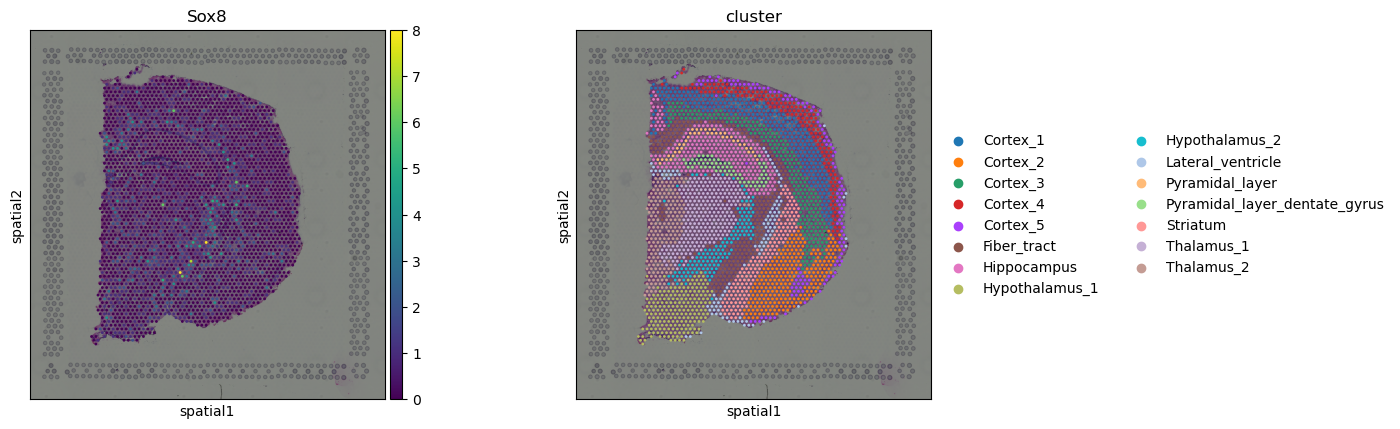
\includegraphics[width=.98\linewidth,height=4.2cm,keepaspectratio]{images/spatial.png}
\end{center}
\vspace{-1mm}
\begin{columns}[t,onlytextwidth]
\begin{column}{.49\textwidth}\small
\bluelabel{左图：Sox8 基因的表达信号}
连续颜色表示该基因的数值高低；结合色条阅读。
\end{column}
\begin{column}{.49\textwidth}\small
\bluelabel{右图：分群及注释标签}
离散颜色区分群体；标签包含分析与解释步骤。
\end{column}\end{columns}
\medskip
{\small 两图使用同一组织的空间位置；圆点是测量位置，不自动等于单个细胞。}

\source{来源：\href{https://www.nature.com/articles/s41592-021-01358-2}{\mbox{Squidpy，2022（DOI: 10.1038/s41592-021-01358-2）}}\par \href{https://squidpy.readthedocs.io/en/latest/notebooks/examples/plotting/plot_scatter.html}{图片：Squidpy / Theis Lab / scverse}；\href{https://github.com/scverse/squidpy/blob/main/LICENSE}{BSD 3-Clause}；原图等比缩放。}
\note{此图来自Squidpy官方Visium教学数据示例，是真实数据的可视化，不是我们前面的肿瘤设问，也不是四位置合成算例。左图连续色条表示Sox8表达信号，右图离散图例显示分群与注释标签。这里不把色条当作未经处理的原始分子数；也不把分群标签说成实验直接读出的细胞身份。先看坐标一致和表达信号空间分布，再看类别解释。}
\end{frame}

% PAGE 55 / 位置让研究问题更具体
\begin{frame}{位置让研究问题更具体}\relax
\begin{itemize}\wideitems
\item 免疫细胞集中在肿瘤边缘，与出现在内部，是不同观察。
\item 脑组织不同结构层可以呈现不同表达模式。
\item 空间关系帮助提出局部环境、边界和邻近关系的问题。
\end{itemize}\keypoint{证据边界}{位置关系可以支持描述和假设，单凭布局不能确证功能或因果。}
\source{来源：\href{https://www.science.org/doi/10.1126/science.aaf2403}{\mbox{St\aa hl等，Science 2016（DOI: 10.1126/science.aaf2403）}}}
\note{把“空间有意义”落实为内部、边缘和组织层等具体问题，而不是抽象地说空间信息很重要。后面的方法必须服务于这些问题。}
\end{frame}

% PAGE 56 / 细胞、spot与bin：三种观测单位
\begin{frame}{细胞、spot与bin：三种观测单位}\relax
\par\noindent{\small\setlength{\tabcolsep}{7pt}\renewcommand{\arraystretch}{1.3}
\begin{tabularx}{\dimexpr\linewidth-4pt\relax}{@{}YYY@{}}\toprule
单位 & 一行可以代表什么 & 需要注意\\\midrule
分割得到的细胞 & 一个细胞区域记录到的RNA & 分割与分子归属可能有误差\\
spot & 一个捕获区域的混合信号 & 可能包含多个细胞\\
bin & 一个合并网格区域的信号 & 网格边界不自动等于细胞边界\\
\bottomrule\end{tabularx}\par}

\source{来源：\href{https://www.science.org/doi/10.1126/science.aaf2403}{\mbox{St\aa hl等，Science 2016（DOI: 10.1126/science.aaf2403）}}\hspace{1em}\allowbreak \href{https://www.10xgenomics.com/spatial-transcriptomics}{\mbox{10x：空间检测技术（10xgenomics.com）}}}
\note{这是全篇必须讲透的一页。可以让听众以后拿到文件先问“一行是什么”。分辨率提高不自动保证每行就是完整细胞，定义来自实验与后续处理。}
\end{frame}

% PAGE 57 / 区域边界与细胞边界
\begin{frame}{区域边界与细胞边界}\relax
\begin{itemize}\wideitems
\item 捕获区域覆盖到什么，与细胞的实际轮廓不是同一个问题。
\item 一个spot可能同时包含肿瘤细胞与免疫细胞。
\item 一个bin可能只覆盖部分细胞，也可能包含多个细胞贡献。
\end{itemize}\keypoint{对注释的影响}{混合表达不适合未经说明就强制赋予单一细胞身份。}
\source{依据：配套讲义第8章。}
\note{此页承上启下，后面P4同时有A、B信号时就要回到测量单位。不要因为算法输出一个类别，就把混合区域变成了真实单细胞。}
\end{frame}

% PAGE 58 / 二维切片与三维组织
\begin{frame}{二维切片与三维组织}\relax
\begin{itemize}\wideitems
\item 常见空间实验测量一张二维组织切片。
\item 二维坐标保留切片内的位置关系。
\item 完整器官的三维结构，通常需要多个切片或其他信息。
\end{itemize}\keypoint{表述范围}{切片内的观察，应先按这张切片的覆盖范围解释。}
\source{依据：配套讲义第8章。}
\note{不必扩展三维重建技术，只提醒观测范围。与最后“单切片能推广到哪里”的问题呼应。}
\end{frame}

\subsection{第9章：位置标签与实验读数}

% PAGE 59 / 第9章：位置标签与实验读数
\begin{frame}{第9章：位置标签与实验读数}\relax
\vfill\begin{center}\begin{minipage}{.86\linewidth}
{\large\color{AcademicBlue}本章导读\par}\vspace{4mm}
{\Large 本章沿着实验读数的形成过程，理解位置条码、UMI、读段与计数各自代表什么。\par\vspace{4mm}弄清这些对应关系，才能正确解释表达矩阵中的数字。\par}
\end{minipage}\end{center}\vfill
\source{依据：配套讲义第9章。}
\note{章节导入。本章沿着实验读数的形成过程，理解位置条码、UMI、读段与计数各自代表什么。弄清这些对应关系，才能正确解释表达矩阵中的数字。}
\end{frame}

% PAGE 60 / 测序路线：用标签关联位置
\begin{frame}{测序路线：用标签关联位置}\relax

\begin{enumerate}\wideitems
  \item 载体上的不同捕获位置具有不同空间条形码。
  \item 放置组织薄片，捕获RNA并经过建库等实验处理。
  \item 测序得到read，识别位置标签与目标序列。
  \item 将信号汇总并关联回组织坐标。
\end{enumerate}
\vspace{3mm}
\keypoint{条形码的作用}{实验知道标签与位置的对应关系，计算流程利用这一关系恢复来源。}

\source{来源：\href{https://www.science.org/doi/10.1126/science.aaf2403}{\mbox{St\aa hl等，Science 2016（DOI: 10.1126/science.aaf2403）}}}
\note{这是典型的空间条形码路线，2016年的经典工作采用了这类思路。说明流程是简化说明，不把某一个平台的具体步骤当作所有空间技术的统一流程。}
\end{frame}

% PAGE 61 / 一份测序读数需要回答什么
\begin{frame}{一份测序读数需要回答什么}\relax
\par\noindent{\small\setlength{\tabcolsep}{7pt}\renewcommand{\arraystretch}{1.3}
\begin{tabularx}{\dimexpr\linewidth-4pt\relax}{@{}YYY@{}}\toprule
问题 & 帮助回答的信息 & 类比\\\midrule
来自哪里？ & 空间条形码与坐标对应表 & 地址标签\\
属于哪个目标？ & 与RNA相关的序列或探针信息 & 内容识别线索\\
\bottomrule\end{tabularx}\par}
\vspace{5mm}\begin{itemize}\wideitems
\item read是测序仪读到的序列片段。
\item 建库是将分子处理为适合测序的材料，不是建立数据库。
\end{itemize}
\source{来源：\href{https://www.genome.gov/genetics-glossary/RNA-seq}{\mbox{NHGRI：RNA-seq（genome.gov）}}\hspace{1em}\allowbreak \href{https://www.science.org/doi/10.1126/science.aaf2403}{\mbox{St\aa hl等，Science 2016（DOI: 10.1126/science.aaf2403）}}}
\note{解释实验常将RNA信息转换到适合建库和测序的DNA产物上。测序仪读到DNA产物不表示本研究对象变成了基因组突变。}
\end{frame}

% PAGE 62 / UMI：识别重复来源的线索
\begin{frame}{UMI：识别重复来源的线索}\relax
\begin{itemize}\wideitems
\item 扩增可以使一个原始分子产生多个副本。
\item 多个reads可能来自同一分子来源。
\item 部分方案加入UMI，帮助识别和合并重复来源。
\end{itemize}\keypoint{两个标签的分工}{空间条形码帮助识别位置；UMI帮助分子去重。}
\source{来源：\href{https://www.10xgenomics.com/support/cn/software/cell-ranger-arc/latest/getting-started/glossary-of-terms}{\mbox{10x：UMI术语（10xgenomics.com）}}}
\note{UMI是独特分子标识符。不能把UMI解释成细胞类型标签，也不能把每个不同UMI绝对等同为一个无误的真实分子，真实流程还涉及测序错误等情况。}
\end{frame}

% PAGE 63 / 教学例子：reads与去重计数
\begin{frame}{教学例子：reads与去重计数}\relax
\par\noindent{\small\setlength{\tabcolsep}{7pt}\renewcommand{\arraystretch}{1.3}
\begin{tabularx}{\dimexpr\linewidth-4pt\relax}{@{}YYYY@{}}\toprule
位置 & 目标 & UMI & read数\\\midrule
P1 & 基因A & u1 & 3\\
P1 & 基因A & u2 & 2\\
P1 & 基因A & u3 & 1\\
\bottomrule\end{tabularx}\par}
\vspace{4mm}\keypoint{按这个简化规则汇总}{共6条reads，可能归并为3个分子来源计数。}
\source{依据：配套讲义第9章。}
\note{这是为了说明去重而新增的教学构造，不是真实实验数据。前提是同位置、同基因、忽略UMI碰撞与序列错误的简化规则。不能用这个例子承诺所有计数都精确等于真实RNA数。}
\end{frame}

% PAGE 64 / 成像路线：直接定位RNA信号
\begin{frame}{成像路线：直接定位RNA信号}\relax
\begin{itemize}\wideitems
\item 使用探针等分子工具识别目标。
\item 通过显微成像与多轮识别等过程定位RNA。
\item 可能先得到分子表，再聚合到细胞或区域。
\end{itemize}\keypoint{分子表的直觉}{某种目标RNA在什么坐标被识别到。}
\source{来源：\href{https://www.10xgenomics.com/spatial-transcriptomics}{\mbox{10x：空间检测技术（10xgenomics.com）}}}
\note{探针先理解为识别特定目标的工具。不必背平台名。关键是数据来源不同，测量名单、分辨率、细胞分割和聚合方式会影响后续分析。}
\end{frame}

% PAGE 65 / 两条实验路线与计算输入
\begin{frame}{两条实验路线与计算输入}\relax
\par\noindent{\small\setlength{\tabcolsep}{7pt}\renewcommand{\arraystretch}{1.3}
\begin{tabularx}{\dimexpr\linewidth-4pt\relax}{@{}YYY@{}}\toprule
路线 & 位置关联方式 & 分析前需要确认\\\midrule
空间条形码测序 & 标签对应已知位置 & 捕获单位、计数流程、坐标\\
原位成像 & 成像识别分子位置 & 面板、定位、分割与聚合规则\\
\bottomrule\end{tabularx}\par}
\vspace{5mm}\keypoint{共同问题}{究竟测了哪些目标，以怎样的单位汇总，保留了什么空间关系？}
\source{来源：\href{https://www.science.org/doi/10.1126/science.aaf2403}{\mbox{St\aa hl等，Science 2016（DOI: 10.1126/science.aaf2403）}}\hspace{1em}\allowbreak \href{https://www.10xgenomics.com/support/cn/software/cell-ranger-arc/latest/getting-started/glossary-of-terms}{\mbox{10x：UMI术语（10xgenomics.com）}}\hspace{1em}\allowbreak \href{https://www.10xgenomics.com/spatial-transcriptomics}{\mbox{10x：空间检测技术（10xgenomics.com）}}}
\note{两种路线都可以服务于空间表达研究，但不能忽略各自测量机制。让听众把注意力从平台名字转到可解释的数据对象。}
\end{frame}

% PAGE 66 / 第二部分回顾：先理解测量，再读取数值
\begin{frame}{第二部分回顾：先理解测量，再读取数值}\relax
\begin{itemize}\wideitems
\item 转录组是RNA集合，实验数据是它的不完整测量。
\item bulk、单细胞与空间测量保留的信息层次不同。
\item 一行可能是细胞、spot或bin，需要查实验与处理记录。
\item reads、去重计数与真实分子数量需要分开理解。
\end{itemize}\keypoint{进入计算前的问题}{现在拿到一个数据文件，应该先检查哪些说明？}
\source{依据：配套讲义第9章。}
\note{可以让听众回答：平台、观测单位、目标基因范围、计数流程和空间坐标。下一部分用P1到P4的具体例子，把这些说明转换成矩阵与关联数据。}
\end{frame}

\section{第三部分：计算分析与科研实践}

% PAGE 67 / 第三部分：计算分析与科研实践
\begin{frame}{第三部分：计算分析与科研实践}\relax
\keypoint{核心问题}{如何将测量变成可解释的输入、算法输出和可信结论？}\begin{itemize}\wideitems
\item 第10--11章：表达矩阵、空间坐标、图像与数据容器。
\item 第12--13章：分析流程与常见算法任务。
\item 第14--15章：完整案例、泛化评估与科学验证。
\end{itemize}
\note{这是连接CS背景与空间转录组研究的主体。强调先解释输入，再选任务，最后决定怎样评估，避免从某个复杂模型倒推研究问题。}
\end{frame}

\subsection{第10章：表达矩阵}

% PAGE 68 / 第10章：表达矩阵
\begin{frame}{第10章：表达矩阵}\relax
\vfill\begin{center}\begin{minipage}{.86\linewidth}
{\large\color{AcademicBlue}本章导读\par}\vspace{4mm}
{\Large 本章把 RNA 测量结果写成表达矩阵，逐一解释行、列、数值与零值的含义。\par\vspace{4mm}通过四位置示例，我们把生物学描述转成可以计算的数据。\par}
\end{minipage}\end{center}\vfill
\source{依据：配套讲义第10章。}
\note{章节导入。本章把 RNA 测量结果写成表达矩阵，逐一解释行、列、数值与零值的含义。通过四位置示例，我们把生物学描述转成可以计算的数据。}
\end{frame}

% PAGE 69 / 表达矩阵：汇总位置与基因的信号
\begin{frame}{表达矩阵：汇总位置与基因的信号}\relax
\par\noindent{\small\setlength{\tabcolsep}{7pt}\renewcommand{\arraystretch}{1.3}
\makebox[\dimexpr\linewidth-4pt\relax][c]{\begin{tabular}{@{}lrrr@{}}\toprule
位置 & 基因A & 基因B & 基因C\\\midrule
P1 & 30 & 2 & 5\\
P2 & 27 & 3 & 8\\
P3 & 3 & 28 & 4\\
P4 & 16 & 17 & 6\\
\bottomrule\end{tabular}}\par}
\vspace{4mm}\begin{itemize}\wideitems
\item A：假设提供上皮相关表达线索。
\item B：假设提供免疫相关表达线索；C：假设与增殖相关。
\end{itemize}
\source{依据：配套讲义第10章；教学构造：A、B、C不是实际基因名，计数不是真实实验结果。}
\note{逐行读出P1到P4。所有计数沿用原讲义，A、B、C不是实际基因名。单个教学代号不能替代真实注释所需的多个标志与参考证据。}
\end{frame}

% PAGE 70 / 一行、一列与一个数字
\begin{frame}{一行、一列与一个数字}\relax

\[
X\in\mathbb{N}_0^{N\times G},\qquad
X_{ig}=\text{观测单位 }i\text{ 对基因 }g\text{ 记录的计数}
\]
\vspace{4mm}
\begin{itemize}\wideitems
\item 本例中，$N=4$个位置，$G=3$个基因。
\item 一行是一个观测单位，一列是一个基因。
\item $X_{1,A}=30$，表示P1对基因A记录的计数为30。
\end{itemize}\keypoint{数字的含义}{30不是“有30个基因A”，也不保证精确对应30个真实RNA分子。}
\source{依据：配套讲义第10章；教学计数，矩阵方向统一为“观测 × 基因”。}
\note{解释非负整数集合含零。强调矩阵表示继承实验单位，换成细胞数据时一行可以是细胞，换成spot数据时就是捕获区域。}
\end{frame}

% PAGE 71 / 原始计数与处理后表达值
\begin{frame}{原始计数与处理后表达值}\relax
\par\noindent{\small\setlength{\tabcolsep}{7pt}\renewcommand{\arraystretch}{1.3}
\begin{tabularx}{\dimexpr\linewidth-4pt\relax}{@{}YYY@{}}\toprule
数据状态 & 常见数值类型 & 解释重点\\\midrule
原始计数 & 非负整数 & 流程记录到的计数\\
总量缩放或取对数后 & 通常为实数 & 经过明确处理的表达表示\\
部分进一步变换的表示 & 可能出现负值 & 须按变换定义解释\\
\bottomrule\end{tabularx}\par}
\vspace{4mm}\keypoint{方向与状态都要核对}{有些文件采用“基因 × 位置”；读取时先查行列与处理记录。}
\source{依据：配套讲义第10章。}
\note{不要看到负数就认定数据错误，也不要把任何叫表达矩阵的对象都当作原始counts。后面模型是否接受某种输入，取决于其定义。}
\end{frame}

% PAGE 72 / 从四行数据读取表达模式
\begin{frame}{从四行数据读取表达模式}\relax
\begin{itemize}\wideitems
\item P1和P2：A较高，B较低。
\item P3：B较高，A较低。
\item P4：A与B都较明显。
\end{itemize}\keypoint{P4的解释取决于单位}{多细胞spot可能包含不同细胞的混合；单个细胞还需考虑共表达、分割和背景。}
\source{依据：配套讲义第10章；教学构造，需结合测量单位解释。}
\note{这是前面观测单位概念的具体应用。明确这些是模式读取与候选解释，不是在给A、B、C建立真实生物学身份。}
\end{frame}

% PAGE 73 / 矩阵中的零与补全问题
\begin{frame}{矩阵中的零与补全问题}\relax
\begin{itemize}\wideitems
\item 零首先表示流程没有记录到对应信号。
\item 实际表达低、捕获不到或测序不足都可能造成零。
\item 全部零不等于生物学上的不存在。
\item 也不能假设所有零都是应该填补的缺失。
\end{itemize}\keypoint{算法选择前}{先弄清零的来源，再考虑是否需要建模或补全。}
\source{依据：配套讲义第10章。}
\note{回扣面板中的未测特征。对初学者强调，补全会引入模型假设，不能因为看到了稀疏矩阵就把所有零都改掉。}
\end{frame}

\subsection{第11章：坐标、图像与文件}

% PAGE 74 / 第11章：坐标、图像与文件
\begin{frame}{第11章：坐标、图像与文件}\relax
\vfill\begin{center}\begin{minipage}{.86\linewidth}
{\large\color{AcademicBlue}本章导读\par}\vspace{4mm}
{\Large 本章把表达矩阵、空间坐标、组织图像与数据文件对应起来。\par\vspace{4mm}重点是理解同一个观测位置如何贯穿不同数据对象，避免错配与配准错误。\par}
\end{minipage}\end{center}\vfill
\source{依据：配套讲义第11章。}
\note{章节导入。本章把表达矩阵、空间坐标、组织图像与数据文件对应起来。重点是理解同一个观测位置如何贯穿不同数据对象，避免错配与配准错误。}
\end{frame}

% PAGE 75 / 空间坐标表与表达矩阵
\begin{frame}{空间坐标表与表达矩阵}\relax

\[
S\in\mathbb{R}^{N\times2},\qquad S_i=(x_i,y_i)
\]
\vspace{3mm}
\par\noindent{\small\setlength{\tabcolsep}{7pt}\renewcommand{\arraystretch}{1.3}
\makebox[\dimexpr\linewidth-4pt\relax][c]{\begin{tabular}{@{}lrr@{}}\toprule
位置ID & $x$ & $y$\\\midrule
P1 & 0 & 0\\
P2 & 1 & 0\\
P3 & 0 & 1\\
P4 & 1 & 1\\
\bottomrule\end{tabular}}\par}
\vspace{4mm}\keypoint{对应关系}{$S$的第$i$行，必须与$X$的第$i$行属于同一个观测单位。}
\source{依据：配套讲义第11章；教学坐标，非真实组织位置。}
\note{坐标沿用原讲义的四个教学位置。强调两个数组行数相同只是必要条件，不能证明行与行对应正确。}
\end{frame}

% PAGE 76 / 位置ID：关联不同信息的键
\begin{frame}{位置ID：关联不同信息的键}\relax
\begin{itemize}\wideitems
\item 表达表、坐标表与观测元数据共享位置ID。
\item 筛选、排序或合并文件后，应重新核对ID顺序。
\item 不能只凭行数相同就直接拼接矩阵与坐标。
\end{itemize}\keypoint{一个典型错误}{表达矩阵删掉某些行后，坐标表未同步筛选，结果仍可能画得很像一张地图。}
\source{依据：配套讲义第11章。}
\note{用数据库关联键的概念解释。最后一句是对讲义ID对应要求的具体操作性展开，并非某个真实数据错误案例。后面空间结论一旦建立在错位关联上，就失去基础。}
\end{frame}

% PAGE 77 / 同一组观测：表达计数与空间地图
\begin{frame}{同一组观测：表达计数与空间地图}\relax

\begin{center}
\begin{tikzpicture}[font=\small,x=.9cm,y=.9cm]
  \node at (2.2,3.45) {表达计数};
  \foreach \x/\lab in {.8/A,1.7/B,2.6/C} \node at (\x+.45,-.25) {\lab};
  \foreach \y/\lab in {2.4/P1,1.6/P2,.8/P3,0/P4} \node[anchor=east] at (.7,\y+.4) {\lab};
  \foreach \x/\y/\v in {.8/2.4/30,1.7/2.4/2,2.6/2.4/5,.8/1.6/27,1.7/1.6/3,2.6/1.6/8,.8/.8/3,1.7/.8/28,2.6/.8/4,.8/0/16,1.7/0/17,2.6/0/6} {
    \pgfmathsetmacro{\shade}{8+2.5*\v}
    \fill[AcademicBlue!\shade!white] (\x,\y) rectangle +(.9,.8);
    \draw[white] (\x,\y) rectangle +(.9,.8);
    \ifnum\v>22 \node[text=white] at (\x+.45,\y+.4) {\v};
    \else \node at (\x+.45,\y+.4) {\v}; \fi
  }
  \begin{scope}[shift={(8,.4)}]
    \node at (1.1,3.05) {空间邻居};
    \draw[gray,thick] (0,0) -- (2.2,0) -- (2.2,2.2) -- (0,2.2) -- cycle;
    \foreach \x/\y/\lab/\col in {0/0/P1/AcademicBlue,2.2/0/P2/AcademicBlue,0/2.2/P3/BlueDark,2.2/2.2/P4/gray} {
      \node[circle,fill=\col,text=white,minimum size=.7cm,inner sep=0pt] at (\x,\y) {\lab};
    }
    \node at (0,-.6) {0}; \node at (2.2,-.6) {1};
    \node at (-.65,0) {0}; \node at (-.65,2.2) {1};
    \node at (1.1,-.95) {$x$}; \node at (-1,1.1) {$y$};
  \end{scope}
\end{tikzpicture}
\end{center}
\keypoint{两张视图，共享位置ID}{左边比较分子特征，右边比较真实位置关系。}

\source{依据：配套讲义第11章；教学构造：颜色只用于区分，连线采用本例定义的邻接规则。}
\note{沿用讲义中的矩阵与空间示意图。连线只表示教学网格的横向或纵向相邻，颜色不代表经过验证的细胞类型。请同时指出P1、P2和P3的对应行与位置。}
\end{frame}

% PAGE 78 / 表达邻居与空间邻居
\begin{frame}{表达邻居与空间邻居}\relax
\par\noindent{\small\setlength{\tabcolsep}{7pt}\renewcommand{\arraystretch}{1.3}
\begin{tabularx}{\dimexpr\linewidth-4pt\relax}{@{}YYY@{}}\toprule
关系 & 本例中的观察 & 回答的问题\\\midrule
表达相似 & P1与P2的A、B、C组合比较接近 & 分子特征像不像？\\
空间相邻 & P1与P3坐标相近，但表达不同 & 组织中近不近？\\
\bottomrule\end{tabularx}\par}
\vspace{5mm}\keypoint{建图或建模时}{必须说明邻居关系来自表达、空间，还是两者的组合。}
\source{依据：配套讲义第11章。}
\note{用前一页图再次口头定位。不要把“近邻”当成无需定义的词，它取决于表示空间、距离和建图规则。此处不引入新的复杂图模型。}
\end{frame}

% PAGE 79 / 组织图像与配准
\begin{frame}{组织图像与配准}\relax
\begin{itemize}\wideitems
\item 组织图像提供形态和结构信息。
\item 配准把表达位置与图像中的位置对齐。
\item 需要检查缩放、方向、原点与坐标单位。
\item 图像像素与物理微米不是同一种单位。
\end{itemize}\keypoint{错误的后果}{真实表达信号可能被画到错误区域，影响内部、边缘等区域判断。}
\source{依据：配套讲义第11章。}
\note{可以举出左右翻转、缩放不一致的直觉例子，但不假装有真实错位图。强调配准是后面把结果叠回组织进行验证的前提。}
\end{frame}

% PAGE 80 / AnnData：带注释的矩阵容器
\begin{frame}{AnnData：带注释的矩阵容器}\relax
\par\noindent{\small\setlength{\tabcolsep}{7pt}\renewcommand{\arraystretch}{1.3}
\begin{tabularx}{\dimexpr\linewidth-4pt\relax}{@{}YY@{}}\toprule
字段 & 常见用途\\\midrule
\codetext{X} & 工作矩阵，通常为观测 × 基因\\
\codetext{obs} & 每个观测的样本ID、QC指标与注释\\
\codetext{var} & 基因名称等基因信息\\
\codetext{obsm} & 与观测对应的坐标或低维数组\\
\codetext{layers} & 相同形状、不同处理状态的表达矩阵\\
\bottomrule\end{tabularx}\par}

\source{来源：\href{https://anndata.readthedocs.io/en/stable/generated/anndata.AnnData.html}{\mbox{AnnData数据对象（anndata.readthedocs.io）}}}
\note{用“矩阵加关联表加附加数组”的文件包理解。H5AD是常用保存格式。这里介绍结构而非某个版本API，不加入未核验的具体函数调用。}
\end{frame}

% PAGE 81 / 文件格式与处理状态
\begin{frame}{文件格式与处理状态}\relax
\begin{itemize}\wideitems
\item 文件叫H5AD，不代表已经完成QC。
\item 字段叫\codetext{raw}，不保证里面就是原始计数。
\item 数据含义应以说明文档和处理记录为准。
\end{itemize}\keypoint{拿到文件后的三个问题}{一行是什么？值经过哪些处理？表达、坐标和图像是否正确对应？}
\source{来源：\href{https://anndata.readthedocs.io/en/stable/generated/anndata.AnnData.html}{\mbox{AnnData数据对象（anndata.readthedocs.io）}}}
\note{为下一章分析流程建立检查清单。文件容器可以保存各种处理阶段的数据，名字不能代替数据来源记录。}
\end{frame}

\subsection{第12章：常见分析流程}

% PAGE 82 / 第12章：常见分析流程
\begin{frame}{第12章：常见分析流程}\relax
\vfill\begin{center}\begin{minipage}{.86\linewidth}
{\large\color{AcademicBlue}本章导读\par}\vspace{4mm}
{\Large 本章按分析顺序介绍质量控制、归一化、特征选择、降维、聚类与注释等步骤。\par\vspace{4mm}每一步都围绕输入是什么、改变了什么，以及结果能怎样解释展开。\par}
\end{minipage}\end{center}\vfill
\source{依据：配套讲义第12章。}
\note{章节导入。本章按分析顺序介绍质量控制、归一化、特征选择、降维、聚类与注释等步骤。每一步都围绕输入是什么、改变了什么，以及结果能怎样解释展开。}
\end{frame}

% PAGE 83 / 分析流程：每一步解决不同问题
\begin{frame}{分析流程：每一步解决不同问题}\relax
\par\noindent{\small\setlength{\tabcolsep}{7pt}\renewcommand{\arraystretch}{1.3}
\begin{tabularx}{\dimexpr\linewidth-4pt\relax}{@{}YY@{}}\toprule
步骤 & 主要目的\\\midrule
QC & 识别可能有问题的观测与输入\\
尺度处理 & 让部分测量总量差异更可比\\
特征选择与降维 & 提取表达差异的主要表示\\
聚类与注释 & 分组，并解释分组可能代表什么\\
空间分析 & 把模式放回组织，检查区域、邻居与边界\\
\bottomrule\end{tabularx}\par}

\source{来源：\href{https://scanpy.readthedocs.io/en/stable/tutorials/basics/clustering.html}{\mbox{Scanpy聚类教程（scanpy.readthedocs.io）}}\hspace{1em}\allowbreak \href{https://www.nature.com/articles/s41592-021-01358-2}{\mbox{Squidpy，2022（DOI: 10.1038/s41592-021-01358-2）}}}
\note{流程不是固定仪式。不同模型可能选择不同输入与处理步骤，必须知道每一步要解决什么问题以及可能改变什么。}
\end{frame}

% PAGE 84 / QC：低信号需要结合背景解释
\begin{frame}{QC：低信号需要结合背景解释}\relax
\begin{itemize}\wideitems
\item 某位置计数极低，可能没有覆盖组织。
\item 也可能是该位置细胞本来较少。
\item 结合组织图像、平台和实验背景判断。
\item QC阈值通常不能不加解释地跨数据照搬。
\end{itemize}
\source{来源：\href{https://scanpy.readthedocs.io/en/stable/tutorials/basics/clustering.html}{\mbox{Scanpy聚类教程（scanpy.readthedocs.io）}}}
\note{强调QC判断不是看到低数值就删除。把计算指标与可见组织结构联系起来，尤其要避免误删有意义的稀疏区域。}
\end{frame}

% PAGE 85 / 总计数：一个直观的QC量
\begin{frame}{总计数：一个直观的QC量}\relax

\[
L_i=\sum_{g=1}^{G}X_{ig}
\]
\vspace{3mm}
\par\noindent{\small\setlength{\tabcolsep}{7pt}\renewcommand{\arraystretch}{1.3}
\makebox[\dimexpr\linewidth-4pt\relax][c]{\begin{tabular}{@{}lrrrr@{}}\toprule
位置 & P1 & P2 & P3 & P4\\\midrule
总计数$L_i$ & 37 & 38 & 35 & 39\\
\bottomrule\end{tabular}}\par}
\vspace{5mm}\keypoint{总量的多种来源}{计数多可能来自更多细胞、更多RNA或更高测量效率，单凭$L_i$难以区分。}
\source{依据：配套讲义第12章；由原讲义教学矩阵计算。}
\note{用原计数逐行相加得到37、38、35、39，强调这是派生的教学计算。总量是有用检查量，但不是细胞数或测量质量的直接同义词。}
\end{frame}

% PAGE 86 / 归一化与log1p：调整数值尺度
\begin{frame}{归一化与log1p：调整数值尺度}\relax

\[
\widetilde X_{ig}=\frac{X_{ig}}{L_i}c,\qquad
Z_{ig}=\log(1+\widetilde X_{ig}),\quad L_i>0
\]
\vspace{3mm}
\begin{itemize}\wideitems
\item $c$是人为设定的统一尺度。
\item 按总量缩放缓解部分总量差异，log1p压缩较大数值。
\item $L_i=0$的观测需要先单独处理。
\end{itemize}\keypoint{适用边界}{这是常见处理方式的示意，不是所有平台和模型的统一配方。}
\source{来源：\href{https://scanpy.readthedocs.io/en/stable/tutorials/basics/clustering.html}{\mbox{Scanpy聚类教程（scanpy.readthedocs.io）}}}
\note{依次解释分母、统一尺度和对数。归一化不能恢复没捕获的分子，也不保证移除所有技术误差。某些模型要求原始计数，不能随意输入Z。}
\end{frame}

% PAGE 87 / 归一化教学演算：P1的基因A
\begin{frame}{归一化教学演算：P1的基因A}\relax

\[
X_{1,A}=30,\quad L_1=30+2+5=37,\quad c=100
\]
\[
\widetilde X_{1,A}=\frac{30}{37}\times100\approx81.08
\]
\[
Z_{1,A}=\ln(1+81.08)\approx4.408
\]
\vspace{3mm}
\keypoint{同一信号，不同数值状态}{30是原计数，81.08是缩放值，4.408是本例自然对数变换值。}

\source{依据：配套讲义第12章；教学演算：由原讲义P1计数计算，$c=100$仅为示例。}
\note{这是为了读懂公式增加的具体演算，c取100只是让计算直观。缩放后的每行和为100，但逐元素取对数后的行和通常不再是100。不要将三个数混作同一输入状态。}
\end{frame}

% PAGE 88 / 高变基因与PCA降维
\begin{frame}{高变基因与PCA降维}\relax
\begin{itemize}\wideitems
\item 高变基因HVG：依据变异特征选出的候选基因。
\item 降维：用较少数值保留重要差异。
\item PCA是常用降维方法。
\end{itemize}\keypoint{解释边界}{高变不自动等于最重要的致病基因；主要变化也可能包括技术因素。}
\source{来源：\href{https://scanpy.readthedocs.io/en/stable/tutorials/basics/clustering.html}{\mbox{Scanpy聚类教程（scanpy.readthedocs.io）}}}
\note{让CS学生把HVG理解为一种特征选择思路，PCA理解为表示步骤。不要把统计变异或主成分大小直接解释成生物学价值。}
\end{frame}

% PAGE 89 / 聚类：先发现表达群体
\begin{frame}{聚类：先发现表达群体}\relax
\begin{itemize}\wideitems
\item 聚类将表达较相似的观测分组。
\item 编号0、1、2只代表算法得到的组。
\item 分组可能反映类型、状态或实验差异。
\end{itemize}\keypoint{聚类之后还要回答}{各组由什么特征区分，它们是否与研究问题有关？}
\source{来源：\href{https://scanpy.readthedocs.io/en/stable/tutorials/basics/clustering.html}{\mbox{Scanpy聚类教程（scanpy.readthedocs.io）}}}
\note{回扣第一部分的类型与状态。此处只建立分组结果的含义，下一页单独讲如何赋予生物解释。}
\end{frame}

% PAGE 90 / 注释：为分组建立生物解释
\begin{frame}{注释：为分组建立生物解释}\relax
\begin{itemize}\wideitems
\item 检查多个标志基因的表达组合。
\item 对照参考数据、已有知识与组织背景。
\item 区分确定标签、候选标签与证据不足的情况。
\end{itemize}\keypoint{关键区别}{聚类负责分组，注释负责解释；算法编号没有自带身份。}
\source{来源：\href{https://scanpy.readthedocs.io/en/stable/tutorials/basics/clustering.html}{\mbox{Scanpy聚类教程（scanpy.readthedocs.io）}}}
\note{最后一项是将讲义证据要求转成实际表述方式。强调有证据不足时可以保留不确定性，不能为了得到完整彩色图而强行命名所有组。}
\end{frame}

% PAGE 91 / 批次差异与生物差异
\begin{frame}{批次差异与生物差异}\relax
\begin{itemize}\wideitems
\item 批次可以来自实验轮次或处理条件差异。
\item 批次分组可能与想研究的生物差异混在一起。
\item 看到清晰分群后，需要检查样本来源与处理背景。
\end{itemize}\keypoint{一个需要追问的问题}{模型分开的到底是细胞类型、状态，还是实验来源？}
\source{依据：配套讲义第12章。}
\note{不把批次校正当作自动解决方案，也不讨论特定算法。重点是研究设计与数据来源说明必须进入解释过程。}
\end{frame}

% PAGE 92 / UMAP坐标与真实空间坐标
\begin{frame}{UMAP坐标与真实空间坐标}\relax
\par\noindent{\small\setlength{\tabcolsep}{7pt}\renewcommand{\arraystretch}{1.3}
\begin{tabularx}{\dimexpr\linewidth-4pt\relax}{@{}YYY@{}}\toprule
坐标 & 如何获得 & 应怎样解释\\\midrule
UMAP二维坐标 & 从高维表达映射得到 & 展示某些表达关系\\
组织空间坐标 & 实验与配准建立 & 描述切片内真实位置\\
\bottomrule\end{tabularx}\par}
\vspace{5mm}\keypoint{不能混用的结论}{表达图上接近的点，在组织里可能相距很远；组织布局要用真实空间坐标。}
\source{来源：\href{https://scanpy.readthedocs.io/en/stable/tutorials/basics/clustering.html}{\mbox{Scanpy聚类教程（scanpy.readthedocs.io）}}\hspace{1em}\allowbreak \href{https://www.nature.com/articles/s41592-021-01358-2}{\mbox{Squidpy，2022（DOI: 10.1038/s41592-021-01358-2）}}}
\note{延续“表达近邻与空间近邻”的区分。不对UMAP的全局距离作额外承诺，只说明它不是物理组织地图。}
\end{frame}

% PAGE 93 / 工具的位置：先知道做什么
\begin{frame}{工具的位置：先知道做什么}\relax
\par\noindent{\small\setlength{\tabcolsep}{7pt}\renewcommand{\arraystretch}{1.3}
\begin{tabularx}{\dimexpr\linewidth-4pt\relax}{@{}YYY@{}}\toprule
工具或对象 & 初步定位 & 学习入口\\\midrule
AnnData / H5AD & 容器与保存格式 & 理解矩阵、元数据和附加数组\\
Scanpy & 表达分析工具 & 预处理、降维、聚类等基础例子\\
Squidpy & 空间图与空间统计等能力 & 把表达结果放回空间分析\\
\bottomrule\end{tabularx}\par}
\vspace{4mm}\keypoint{学习顺序}{先解释每一步的目的，再学习函数和参数。}
\source{来源：\href{https://anndata.readthedocs.io/en/stable/generated/anndata.AnnData.html}{\mbox{AnnData数据对象（anndata.readthedocs.io）}}\hspace{1em}\allowbreak \href{https://scanpy.readthedocs.io/en/stable/tutorials/basics/clustering.html}{\mbox{Scanpy聚类教程（scanpy.readthedocs.io）}}\hspace{1em}\allowbreak \href{https://www.nature.com/articles/s41592-021-01358-2}{\mbox{Squidpy，2022（DOI: 10.1038/s41592-021-01358-2）}}}
\note{工具和文档会随版本更新。本汇报保留原讲义给出的来源，不展示特定版本的可执行代码，因此学习时要结合自己所用版本。}
\end{frame}

\subsection{第13章：算法研究任务}

% PAGE 94 / 第13章：算法研究任务
\begin{frame}{第13章：算法研究任务}\relax
\vfill\begin{center}\begin{minipage}{.86\linewidth}
{\large\color{AcademicBlue}本章导读\par}\vspace{4mm}
{\Large 本章把空间转录组中的生物学问题转成具体算法任务，辨认各类方法的输入与输出。\par\vspace{4mm}据此判断不同方法回答的是哪一个问题，以及结果还需要哪些证据。\par}
\end{minipage}\end{center}\vfill
\source{依据：配套讲义第13章。}
\note{章节导入。本章把空间转录组中的生物学问题转成具体算法任务，辨认各类方法的输入与输出。据此判断不同方法回答的是哪一个问题，以及结果还需要哪些证据。}
\end{frame}

% PAGE 95 / 五类问题，五种输出
\begin{frame}{五类问题，五种输出}\relax
\par\noindent{\small\setlength{\tabcolsep}{7pt}\renewcommand{\arraystretch}{1.3}
\begin{tabularx}{\dimexpr\linewidth-4pt\relax}{@{}YYY@{}}\toprule
研究问题 & 输出对象 & CS任务直觉\\\midrule
组织有哪些区域？ & 空间域标签 & 聚类、分割、表征学习\\
混合区域有什么细胞？ & 类型丰度、贡献或比例 & 混合信号分解\\
图像能否预测表达？ & 预测表达向量 & 多输出回归、多模态学习\\
哪些表达随空间变化？ & 空间变异基因或模式 & 空间统计与模式分析\\
哪些细胞可能相互影响？ & 候选通信关系 & 结合知识的关系推断\\
\bottomrule\end{tabularx}\par}

\source{来源：\href{https://www.nature.com/articles/s41592-021-01358-2}{\mbox{Squidpy，2022（DOI: 10.1038/s41592-021-01358-2）}}\hspace{1em}\allowbreak \href{https://www.nature.com/articles/s41587-021-01139-4}{\mbox{cell2location，2022（DOI: 10.1038/s41587-021-01139-4）}}\hspace{1em}\allowbreak \href{https://www.nature.com/articles/s41467-021-21246-9}{\mbox{CellChat，2021（DOI: 10.1038/s41467-021-21246-9）}}}
\note{先讲输出而不是算法名。强调每个任务回答的问题不同，不能用同一个漂亮聚类图替代所有生物学问题。}
\end{frame}

% PAGE 96 / 空间域：组织区域的划分
\begin{frame}{空间域：组织区域的划分}\relax
\begin{itemize}\wideitems
\item 空间域描述组织中结构或表达不同的区域。
\item 例如组织层、肿瘤内部或边缘等区域。
\item 一个区域可以包含多类细胞。
\item 同一种细胞也可能出现在多个区域。
\end{itemize}\keypoint{输出的含义}{区域标签回答“这里属于什么区域”，不必然回答“这里是哪种细胞”。}
\source{来源：\href{https://www.nature.com/articles/s41592-021-01358-2}{\mbox{Squidpy，2022（DOI: 10.1038/s41592-021-01358-2）}}}
\note{回扣观测单位与细胞类型概念。空间域可以与病理区域相关，但不能默认算法每个簇都对应一个真实解剖区域。}
\end{frame}

% PAGE 97 / 空间平滑与真实边界
\begin{frame}{空间平滑与真实边界}\relax
\begin{itemize}\wideitems
\item 空间相邻的位置可能具有相近表达。
\item 也可能刚好位于真实组织边界两侧。
\item 过强平滑可能抹掉有意义的边界。
\end{itemize}\keypoint{评价重点}{除了标签是否连贯，还应检查边界与图像、标志表达和研究问题是否一致。}
\source{依据：配套讲义第13章。}
\note{算法偏好连续区域是建模假设，而不是永远成立的生物事实。指出仅凭空间图看起来平滑不能断言结果更正确。}
\end{frame}

% PAGE 98 / 反卷积：推断混合信号的组成
\begin{frame}{反卷积：推断混合信号的组成}\relax
\begin{itemize}\wideitems
\item 多细胞spot中的表达可能由不同细胞类型共同贡献。
\item 单细胞参考可以提供不同类型的大致表达模板。
\item 反卷积利用混合信号与参考，推断不同成分。
\end{itemize}\keypoint{类比}{已知不同乐器的大致音色，尝试分辨混合声音中各自的贡献。}
\source{来源：\href{https://www.nature.com/articles/s41587-021-01139-4}{\mbox{cell2location，2022（DOI: 10.1038/s41587-021-01139-4）}}}
\note{类比帮助理解混合分解，不意味着真实RNA混合一定严格满足最简单的线性模型。cell2location是相关方法示例，详细机制超出本入门汇报。}
\end{frame}

% PAGE 99 / 反卷积输出的单位与解释
\begin{frame}{反卷积输出的单位与解释}\relax
\par\noindent{\small\setlength{\tabcolsep}{7pt}\renewcommand{\arraystretch}{1.3}
\begin{tabularx}{\dimexpr\linewidth-4pt\relax}{@{}YYY@{}}\toprule
输出名称 & 可能表示什么 & 需要查什么\\\midrule
类型丰度 & 某类成分的估计强度或丰度 & 方法的具体定义\\
相对贡献 & 对混合表达信号的相对贡献 & 是否是RNA层面的贡献\\
比例 & 按某种分母归一化的结果 & 是否真的可解释为细胞比例\\
\bottomrule\end{tabularx}\par}
\vspace{4mm}\keypoint{重要边界}{RNA贡献比例不自动等于细胞数量比例。}
\source{来源：\href{https://www.nature.com/articles/s41587-021-01139-4}{\mbox{cell2location，2022（DOI: 10.1038/s41587-021-01139-4）}}}
\note{P4同时有A、B时，一个混合解释可能合理，但推断多少细胞、多少RNA贡献是不同问题。把输出单位写清楚比只看颜色强弱更重要。}
\end{frame}

% PAGE 100 / 图像预测表达：多模态学习
\begin{frame}{图像预测表达：多模态学习}\relax
\begin{itemize}\wideitems
\item 输入：组织图像块。
\item 输出：一组基因的预测表达值。
\item 从CS看，可对应多输出回归或多模态学习。
\end{itemize}\keypoint{观测与预测区分}{模型利用形态与表达的统计关联，预测值不能当作新完成的RNA实验。}
\source{依据：配套讲义第13章。}
\note{把直接测量的表达与模型预测画出清晰边界。即便预测与实测相关，也要检查测试划分与研究目标，后面评估章节会进一步展开。}
\end{frame}

% PAGE 101 / HVG与SVG：变异与空间规律
\begin{frame}{HVG与SVG：变异与空间规律}\relax
\par\noindent{\small\setlength{\tabcolsep}{7pt}\renewcommand{\arraystretch}{1.3}
\begin{tabularx}{\dimexpr\linewidth-4pt\relax}{@{}YYY@{}}\toprule
概念 & 关注什么 & 不能直接等同\\\midrule
高变基因HVG & 表达值的变异特征 & 有组织的空间模式\\
空间变异基因SVG & 表达与空间位置的关联模式 & 任意数值波动\\
\bottomrule\end{tabularx}\par}
\vspace{5mm}\keypoint{直觉比较}{表达变化很大但位置随机，与沿组织呈现梯度，是不同现象。}
\source{来源：\href{https://www.nature.com/articles/s41592-021-01358-2}{\mbox{Squidpy，2022（DOI: 10.1038/s41592-021-01358-2）}}}
\note{不要简单说HVG与SVG互斥，它们关注维度不同，同一基因可能同时具备某些特征。此处重点是区分变异大小与空间结构。}
\end{frame}

% PAGE 102 / 候选细胞通信：表达、空间与已有知识
\begin{frame}{候选细胞通信：表达、空间与已有知识}\relax
\begin{itemize}\wideitems
\item 配体是参与信号传递、可与受体结合的分子等。
\item 受体是接收相关信号的分子组件。
\item 算法结合表达、空间关系和配体受体知识提出候选联系。
\end{itemize}\keypoint{方法示例}{CellChat是细胞通信推断的相关框架之一。}
\source{来源：\href{https://www.nature.com/articles/s41467-021-21246-9}{\mbox{CellChat，2021（DOI: 10.1038/s41467-021-21246-9）}}}
\note{不要暗示所有通信方法都必须使用空间信息，或CellChat的所有设置都默认使用空间。这里只说空间研究可以结合这些信息提出候选关系。}
\end{frame}

% PAGE 103 / 通信候选与机制证据
\begin{frame}{通信候选与机制证据}\relax
\par\noindent{\small\setlength{\tabcolsep}{7pt}\renewcommand{\arraystretch}{1.3}
\begin{tabularx}{\dimexpr\linewidth-4pt\relax}{@{}YY@{}}\toprule
已有证据 & 能支持的初步表述\\\midrule
空间靠近 & 具备邻近关系\\
相关RNA共表达 & 存在表达层面的候选线索\\
蛋白、下游变化或干预证据 & 进一步检验通信与机制假设\\
\bottomrule\end{tabularx}\par}
\vspace{4mm}\keypoint{结论边界}{邻近或共表达本身，不是通信确实发生的完整证明。}
\source{来源：\href{https://www.nature.com/articles/s41467-021-21246-9}{\mbox{CellChat，2021（DOI: 10.1038/s41467-021-21246-9）}}}
\note{回扣RNA不等于蛋白质与功能。候选网络的作用是组织假设、指导检验，不是把漂亮网络图直接当成机制结论。}
\end{frame}

\subsection{第14章：贯穿案例与科研流程}

% PAGE 104 / 第14章：贯穿案例与科研流程
\begin{frame}{第14章：贯穿案例与科研流程}\relax
\vfill\begin{center}\begin{minipage}{.86\linewidth}
{\large\color{AcademicBlue}本章导读\par}\vspace{4mm}
{\Large 本章回到肿瘤切片中的免疫细胞分布问题，把提问、数据分析与验证串成研究流程。\par\vspace{4mm}通过数量、密度和比例的比较，说明指标定义如何影响结论。\par}
\end{minipage}\end{center}\vfill
\source{依据：配套讲义第14章。}
\note{章节导入。本章回到肿瘤切片中的免疫细胞分布问题，把提问、数据分析与验证串成研究流程。通过数量、密度和比例的比较，说明指标定义如何影响结论。}
\end{frame}

% PAGE 105 / 完整案例：免疫细胞主要在哪里
\begin{frame}{完整案例：免疫细胞主要在哪里}\relax
\begin{itemize}\wideitems
\item 问题：这张肿瘤切片中，免疫细胞主要在内部还是边缘？
\item 先确认测量单位与免疫相关表达、参考证据。
\item 再定义区域、选方法、比较指标并验证。
\end{itemize}\keypoint{案例路线}{测量、推断、比较、验证、解释，各自承担不同任务。}
\source{依据：配套讲义第14章。}
\note{现在重新提出开头的问题。听众已经知道细胞、测量和矩阵，此时可以完整走一遍研究过程，不需要从模型结构开始。}
\end{frame}

% PAGE 106 / 第一步：分清观测与推断
\begin{frame}{第一步：分清观测与推断}\relax
\par\noindent{\small\setlength{\tabcolsep}{7pt}\renewcommand{\arraystretch}{1.3}
\begin{tabularx}{\dimexpr\linewidth-4pt\relax}{@{}YY@{}}\toprule
层次 & 本案例中的内容\\\midrule
直接观测 & 记录到的RNA信号、位置及组织形态\\
基于观测的推断 & 细胞身份、某类细胞的丰度或贡献\\
进一步比较与解释 & 内部与边缘的分布差异及其可能原因\\
\bottomrule\end{tabularx}\par}
\vspace{4mm}\keypoint{表述时的关键}{“这个位置记录到信号”和“这里有多少免疫细胞”往往不属于同一层证据。}
\source{依据：配套讲义第14章。}
\note{请听众指出哪一步需要注释，哪一步可能需要反卷积。避免把模型输出当成仪器直接读数。}
\end{frame}

% PAGE 107 / 第二步：定义内部与边缘
\begin{frame}{第二步：定义内部与边缘}\relax
\begin{itemize}\wideitems
\item 说明区域来自专家图像标注，还是其他有依据的分析。
\item 记录边界如何确定，以及它可能存在的不确定性。
\item 明确哪些位置或细胞被分配到每个区域。
\end{itemize}\keypoint{比较必须有参照}{“更多在内部”只有在内部、边缘被清楚定义后才有可检验含义。}
\source{依据：配套讲义第14章。}
\note{区域定义影响比较对象。专家标注是有价值参照，但也可能不确定，不能把所有参照一概看成完美真值。}
\end{frame}

% PAGE 108 / 第三步：按测量单位选择方法
\begin{frame}{第三步：按测量单位选择方法}\relax
\par\noindent{\small\setlength{\tabcolsep}{7pt}\renewcommand{\arraystretch}{1.3}
\begin{tabularx}{\dimexpr\linewidth-4pt\relax}{@{}YYY@{}}\toprule
数据单位 & 可考虑的分析 & 需要保留的限制\\\midrule
有依据注释的细胞 & 按区域统计细胞分布 & 注释与分割误差\\
多细胞spot & 必要时推断类型丰度或贡献 & 混合与参考不确定性\\
bin区域 & 按网格定义解释表达或组成 & 不自动等于完整细胞\\
\bottomrule\end{tabularx}\par}
\vspace{4mm}\keypoint{不能跨越的步骤}{不能只凭单一类别标签，把混合spot当成一个真实细胞。}
\source{依据：配套讲义第14章。}
\note{将第八章与第十三章连接起来。具体方法取决于测量对象和问题，而不是所有数据都套同一个注释流程。}
\end{frame}

% PAGE 109 / 第四步：为“更多”选择分母
\begin{frame}{第四步：为“更多”选择分母}\relax

\[
\text{免疫细胞密度}_r=\frac{n_{\mathrm{immune},r}}{A_r}
\]
\[
\text{免疫细胞比例}_r=\frac{n_{\mathrm{immune},r}}{n_{\mathrm{all},r}}
\]
\begin{itemize}\wideitems
\item $A_r$：区域面积；$n_{\mathrm{all},r}$：区域总细胞数。
\item 密度回答单位面积有多少；比例回答细胞中占多少。
\item 分母须大于零，且输入必须可按细胞数量解释。
\end{itemize}
\source{依据：配套讲义第14章。}
\note{总数量、单位面积密度和细胞比例是三种不同问题。若方法输出RNA相对贡献，就不能直接代入细胞数公式。}
\end{frame}

% PAGE 110 / 教学演算：总数、密度与比例
\begin{frame}{教学演算：总数、密度与比例}\relax
\par\noindent{\small\setlength{\tabcolsep}{7pt}\renewcommand{\arraystretch}{1.3}
\makebox[\dimexpr\linewidth-4pt\relax][c]{\begin{tabular}{@{}lrrr@{}}\toprule
区域 & 免疫细胞数 & 总细胞数 & 面积\\\midrule
内部 & 100 & 1000 & $10\,\mathrm{mm}^2$\\
边缘 & 60 & 200 & $2\,\mathrm{mm}^2$\\
\bottomrule\end{tabular}}\par}

\vspace{4mm}
\begin{itemize}\compactitems
  \item 内部总数更多：$100>60$。
  \item 边缘密度更高：$30>10$ 个/$\mathrm{mm}^2$。
  \item 边缘比例更高：$30\%>10\%$。
\end{itemize}

\source{依据：配套讲义第14章；新增教学数值，仅为指标演算；不是实际肿瘤样本结果。}
\note{新增教学构造，用来具体说明分母会改变“更多”的含义。内部100除10得到10，边缘60除2得到30；比例分别100除1000和60除200。它们不矛盾，而是在回答不同问题。}
\end{frame}

% PAGE 111 / 第五步：把结果放回组织检查
\begin{frame}{第五步：把结果放回组织检查}\relax
\begin{itemize}\wideitems
\item 将注释或丰度结果画回真实空间位置。
\item 检查是否与组织形态、标志表达及区域定义相符。
\item 比较预先明确的数量、密度、比例或方法定义的丰度。
\item 观察结论是否依赖某个边界、注释或处理选择。
\end{itemize}
\source{依据：配套讲义第14章。}
\note{最后一项是对讲义验证要求的操作性展开：可以检查合理替代选择下描述是否仍成立。不能只说结果看起来符合直觉，也要说明相符的证据。}
\end{frame}

% PAGE 112 / 第六步：决定结论可以推广到哪里
\begin{frame}{第六步：决定结论可以推广到哪里}\relax
\par\noindent{\small\setlength{\tabcolsep}{7pt}\renewcommand{\arraystretch}{1.3}
\begin{tabularx}{\dimexpr\linewidth-4pt\relax}{@{}YYY@{}}\toprule
目标 & 现有切片能支持什么 & 还需要什么\\\midrule
描述这张切片 & 本切片内的观测与推断结果 & 相应标注、测量和方法依据\\
推广到患者群体 & 单张切片通常不够 & 更多独立供体与合适设计\\
解释形成机制 & 分布可以提出机制假设 & 机制、干预等更强证据\\
\bottomrule\end{tabularx}\par}

\source{依据：配套讲义第14章。}
\note{将样本内描述、群体泛化和因果机制分开。此页为下一章的供体划分和独立样本概念铺垫。}
\end{frame}

\subsection{第15章：可信结论与评估}

% PAGE 113 / 第15章：可信结论与评估
\begin{frame}{第15章：可信结论与评估}\relax
\vfill\begin{center}\begin{minipage}{.86\linewidth}
{\large\color{AcademicBlue}本章导读\par}\vspace{4mm}
{\Large 本章讨论怎样评估分析结果，重点检查独立样本、数据划分、对照与验证依据。\par\vspace{4mm}我们将区分观察到的关联、可以推广的结果与仍待检验的机制解释。\par}
\end{minipage}\end{center}\vfill
\source{依据：配套讲义第15章。}
\note{章节导入。本章讨论怎样评估分析结果，重点检查独立样本、数据划分、对照与验证依据。我们将区分观察到的关联、可以推广的结果与仍待检验的机制解释。}
\end{frame}

% PAGE 114 / 大量位置与独立供体
\begin{frame}{大量位置与独立供体}\relax
\begin{itemize}\wideitems
\item 一名患者的一张切片可以包含大量观测位置。
\item 这些位置共享供体、局部环境与部分实验过程。
\item 数千个spot不能当作数千名独立患者。
\end{itemize}\keypoint{独立样本单位}{供体是提供组织样本的个体；评估和统计推断都要说明独立单位。}
\source{依据：配套讲义第15章。}
\note{数量多不自动等于证据独立。对CS听众强调数据行数与研究层面的独立样本数是两个不同概念。}
\end{frame}

% PAGE 115 / 训练与测试划分应对应泛化目标
\begin{frame}{训练与测试划分应对应泛化目标}\relax
\par\noindent{\small\setlength{\tabcolsep}{7pt}\renewcommand{\arraystretch}{1.3}
\begin{tabularx}{\dimexpr\linewidth-4pt\relax}{@{}YYY@{}}\toprule
目标 & 需要关注的划分 & 不能自动宣称\\\midrule
同切片内插值 & 同切片中留出部分位置 & 对新患者泛化\\
新切片预测 & 按切片留出并说明供体关系 & 切片不同就等于供体不同\\
未见患者泛化 & 按供体划分 & 同患者不同切片属于未见患者\\
\bottomrule\end{tabularx}\par}

\source{依据：配套讲义第15章。}
\note{不给出唯一适合所有任务的划分方式。随机留出相邻位置可以研究插值，但结论要准确描述；想验证新患者就必须处理供体层面的独立性。}
\end{frame}

% PAGE 116 / 信息泄漏与可使用的数据范围
\begin{frame}{信息泄漏与可使用的数据范围}\relax
\begin{itemize}\wideitems
\item 特征选择、参考构建和调参可能接触测试信息。
\item 需要记录这些步骤使用了哪些数据。
\item 允许无标签目标数据，与完全不接触目标数据，是不同设置。
\end{itemize}\keypoint{评估协议需要写清}{数据可见范围、处理步骤和调参依据，要与最终泛化表述一致。}
\source{依据：配套讲义第15章。}
\note{不要把所有使用目标无标签数据的情况都一概视为错误；关键是协议是否允许、是否清楚报告，以及它回答什么问题。}
\end{frame}

% PAGE 117 / 参照标签与真值的证据强度
\begin{frame}{参照标签与真值的证据强度}\relax
\par\noindent{\small\setlength{\tabcolsep}{7pt}\renewcommand{\arraystretch}{1.3}
\begin{tabularx}{\dimexpr\linewidth-4pt\relax}{@{}YYY@{}}\toprule
参照来源 & 能提供什么 & 需要留意\\\midrule
专家区域标注 & 专业判断形成的区域参照 & 边界与判断不确定性\\
独立实测 & 另一种观测证据 & 测量自身的范围和误差\\
已有算法输出 & 与已有结果比较的依据 & 可能继承已有方法偏差\\
\bottomrule\end{tabularx}\par}
\vspace{4mm}\keypoint{评价解释}{更像已有算法，不必然表示更接近真实生物状态。}
\source{依据：配套讲义第15章。}
\note{Ground truth常译为真值，但实际参照强弱不同。鼓励论文阅读时追问标签是怎样获得的，而不是只记住指标名字。}
\end{frame}

% PAGE 118 / 差异表达：发现组间表达差异
\begin{frame}{差异表达：发现组间表达差异}\relax
\begin{itemize}\wideitems
\item 两组中某个基因表达不同，可以称为差异表达现象。
\item 差异可能来自细胞组成、状态或测量方式。
\item 差异表达为后续研究提供线索。
\end{itemize}\keypoint{表述边界}{观察到差异，不直接证明该基因导致了某种现象。}
\source{依据：配套讲义第15章。}
\note{将组成变化与单细胞状态变化联系回bulk的例子。不要用表达差异自动解释调控机制。}
\end{frame}

% PAGE 119 / FDR、差异幅度与生物学解释
\begin{frame}{FDR、差异幅度与生物学解释}\relax
\begin{itemize}\wideitems
\item 大量基因检验需要考虑多重检验问题。
\item FDR用于控制假发现率相关问题。
\item FDR不能代替差异幅度和生物学解释。
\item 它不应直接解释为某个具体结论为假的概率。
\end{itemize}
\source{依据：配套讲义第15章。}
\note{保留讲义中的关键限定，不在此引入没有数据支持的显著性数值。若继续深入统计，应另学检验假设与具体方法条件。}
\end{frame}

% PAGE 120 / 相关观察与因果机制
\begin{frame}{相关观察与因果机制}\relax
\par\noindent{\small\setlength{\tabcolsep}{7pt}\renewcommand{\arraystretch}{1.3}
\begin{tabularx}{\dimexpr\linewidth-4pt\relax}{@{}YY@{}}\toprule
表述层次 & 例子\\\midrule
描述 & 某切片的某区域出现更明显的表达信号\\
关联 & 某表达模式与位置或状态相关\\
机制假设 & 某过程可能参与形成该分布\\
因果判断 & 需要与问题匹配的更强证据，例如合适干预\\
\bottomrule\end{tabularx}\par}
\vspace{4mm}\keypoint{写结论时}{让动词与证据匹配：观察到、提示、支持假设与证明因果具有不同强度。}
\source{依据：配套讲义第15章。}
\note{这不是说观察研究没有价值，而是要求准确命名结果。回扣开头不凭分布直接判断治疗效果的限制。}
\end{frame}

% PAGE 121 / 读论文与设计研究的五个问题
\begin{frame}{读论文与设计研究的五个问题}\relax

\begin{enumerate}\wideitems
  \item 研究哪种组织，回答什么生物问题？
  \item 一行是什么，表达值怎样得到？
  \item 模型输出是直接观测，还是推断？
  \item 用什么参照与独立数据验证？
  \item 相比简单方法，具体解决了哪个困难？
\end{enumerate}

\source{依据：配套讲义第15章。}
\note{建议视频录制时逐项用贯穿案例作答。最后一项让CS学生关注方法带来的实际研究价值，而不是仅比较模型复杂度。}
\end{frame}

% PAGE 122 / 第三部分回顾：数据到结论的证据链
\begin{frame}{第三部分回顾：数据到结论的证据链}\relax
\par\noindent{\small\setlength{\tabcolsep}{7pt}\renewcommand{\arraystretch}{1.3}
\begin{tabularx}{\dimexpr\linewidth-4pt\relax}{@{}YY@{}}\toprule
环节 & 需要讲清楚的内容\\\midrule
测量 & 观测单位、目标范围、数值来源\\
表示 & 矩阵、坐标、图像与ID对应\\
任务 & 输出对象与输入证据\\
验证 & 参照来源、独立单位与泛化目标\\
解释 & 结论范围与仍待检验的假设\\
\bottomrule\end{tabularx}\par}

\source{依据：配套讲义第15章。}
\note{最后将第三部分连成完整链条。可以请听众从组织薄片开始，用自己的话依次说出五个环节。下一部分用于术语回查和继续学习。}
\end{frame}

\section{第四部分：术语回查与延伸阅读}

% PAGE 123 / 第四部分：术语回查与延伸阅读
\begin{frame}{第四部分：术语回查与延伸阅读}\relax
\begin{itemize}\wideitems
\item 第16章：按主题回查术语与常见混淆。
\item 第17章：安排下一步学习，查阅基础资料与分析文档。
\end{itemize}\keypoint{使用方式}{先把主线讲清楚，再按需要回查名词，不必一次背完所有术语。}
\note{这一部分适合作为视频的回顾与学习建议。术语表按主题分多页，观众也可以在后续学习中直接返回对应页。}
\end{frame}

\subsection{第16章：核心术语回查}

% PAGE 124 / 第16章：核心术语回查
\begin{frame}{第16章：核心术语回查}\relax
\vfill\begin{center}\begin{minipage}{.86\linewidth}
{\large\color{AcademicBlue}本章导读\par}\vspace{4mm}
{\Large 本章按研究对象、分子过程、测量与计算任务回查核心术语和常见混淆。\par\vspace{4mm}把相近概念放在一起比较，帮助听众回顾前文并在后续学习时快速查找。\par}
\end{minipage}\end{center}\vfill
\source{依据：配套讲义第16章。}
\note{章节导入。本章按研究对象、分子过程、测量与计算任务回查核心术语和常见混淆。把相近概念放在一起比较，帮助听众回顾前文并在后续学习时快速查找。}
\end{frame}

% PAGE 125 / 术语回查：研究对象与分子
\begin{frame}{术语回查：研究对象与分子}\relax
\par\noindent{\small\setlength{\tabcolsep}{7pt}\renewcommand{\arraystretch}{1.3}
\begin{tabularx}{\dimexpr\linewidth-4pt\relax}{@{}YYY@{}}\toprule
术语 & 最初的理解 & 常见混淆\\\midrule
细胞 Cell & 结构与功能的基本单位 & 空间数据一行不一定是细胞\\
组织 Tissue & 细胞与周围材料形成的结构 & 包含布局与结构关系\\
DNA & 保存遗传信息的分子 & 转录不把DNA全部变成RNA\\
基因 Gene & DNA上的功能区段 & 存在不等于当前高表达\\
RNA / mRNA & RNA与其中的信使RNA & 部分RNA本身有功能\\
蛋白质 Protein & 氨基酸链形成的分子 & RNA量不直接等于蛋白量\\
\bottomrule\end{tabularx}\par}

\source{来源：\href{https://www.cancer.gov/publications/dictionaries/cancer-terms/def/organ}{\mbox{NCI：器官（cancer.gov）}}\hspace{1em}\allowbreak \href{https://www.genome.gov/genetics-glossary/Deoxyribonucleic-Acid-DNA}{\mbox{NHGRI：DNA（genome.gov）}}\hspace{1em}\allowbreak \href{https://www.genome.gov/genetics-glossary}{\mbox{NHGRI：基础术语（genome.gov）}}\hspace{1em}\allowbreak \href{https://www.genome.gov/genetics-glossary/Transcription}{\mbox{NHGRI：转录（genome.gov）}}\hspace{1em}\allowbreak \href{https://www.genome.gov/genetics-glossary/Messenger-RNA-mRNA}{\mbox{NHGRI：mRNA（genome.gov）}}\hspace{1em}\allowbreak \href{https://www.genome.gov/genetics-glossary/Protein}{\mbox{NHGRI：蛋白质（genome.gov）}}\hspace{1em}\allowbreak \href{https://www.genome.gov/genetics-glossary/Translation}{\mbox{NHGRI：翻译（genome.gov）}}\hspace{1em}\allowbreak \href{https://www.genome.gov/genetics-glossary/Gene-Expression}{\mbox{NHGRI：基因表达（genome.gov）}}}
\note{这页回查第一部分的对象层次。建议视频中不逐字重复定义，而是针对听众最容易混淆的列进行回顾。}
\end{frame}

% PAGE 126 / 术语回查：信息使用与细胞解释
\begin{frame}{术语回查：信息使用与细胞解释}\relax
\par\noindent{\small\setlength{\tabcolsep}{7pt}\renewcommand{\arraystretch}{1.3}
\begin{tabularx}{\dimexpr\linewidth-4pt\relax}{@{}YYY@{}}\toprule
术语 & 最初的理解 & 常见混淆\\\midrule
转录与翻译 & 制造RNA、按mRNA制造蛋白质 & 属于不同步骤\\
基因组与转录组 & 保存的信息、当时RNA集合 & 信息与状态不同\\
转录本 Transcript & 转录产生的RNA产物 & 同一基因可以有不同版本\\
基因表达 & 信息被用于产生功能产物 & RNA语境常指相关信号\\
细胞类型与状态 & 相对身份、当前活动 & 聚类可能反映不同因素\\
标志基因 Marker & 身份或状态的表达线索 & 单个标志通常不够\\
\bottomrule\end{tabularx}\par}

\source{来源：\href{https://www.genome.gov/genetics-glossary}{\mbox{NHGRI：基础术语（genome.gov）}}\hspace{1em}\allowbreak \href{https://www.genome.gov/genetics-glossary/Transcription}{\mbox{NHGRI：转录（genome.gov）}}\hspace{1em}\allowbreak \href{https://www.genome.gov/genetics-glossary/Messenger-RNA-mRNA}{\mbox{NHGRI：mRNA（genome.gov）}}\hspace{1em}\allowbreak \href{https://www.genome.gov/genetics-glossary/Protein}{\mbox{NHGRI：蛋白质（genome.gov）}}\hspace{1em}\allowbreak \href{https://www.genome.gov/genetics-glossary/Translation}{\mbox{NHGRI：翻译（genome.gov）}}\hspace{1em}\allowbreak \href{https://www.genome.gov/genetics-glossary/Gene-Expression}{\mbox{NHGRI：基因表达（genome.gov）}}\hspace{1em}\allowbreak \href{https://www.genome.gov/about-genomics/fact-sheets/Transcriptome-Fact-Sheet}{\mbox{NHGRI：转录组（genome.gov）}}}
\note{重点回顾类型、状态和标志基因的关系。对于CS读者，特征与标签之间不是天然一一对应，而要借助背景与参考建立解释。}
\end{frame}

% PAGE 127 / 术语回查：测量与计数
\begin{frame}{术语回查：测量与计数}\relax
\par\noindent{\small\setlength{\tabcolsep}{7pt}\renewcommand{\arraystretch}{1.3}
\begin{tabularx}{\dimexpr\linewidth-4pt\relax}{@{}YYY@{}}\toprule
术语 & 最初的理解 & 常见混淆\\\midrule
Panel & 预选基因名单 & 未测特征不等于零表达\\
Bulk / scRNA-seq & 混合与单细胞RNA测量 & 总体与个体差异不同\\
Spot / bin & 捕获区域、合并网格 & 不自动对应完整细胞\\
Barcode / UMI & 位置等标签、去重线索 & UMI不用于标注细胞类型\\
Read / count & 序列读段、汇总计数 & 多个reads可能来源相同\\
Counts / 归一化值 & 计数、尺度处理后的值 & 须按处理状态解释\\
\bottomrule\end{tabularx}\par}

\source{来源：\href{https://www.genome.gov/genetics-glossary/RNA-seq}{\mbox{NHGRI：RNA-seq（genome.gov）}}\hspace{1em}\allowbreak \href{https://www.science.org/doi/10.1126/science.aaf2403}{\mbox{St\aa hl等，Science 2016（DOI: 10.1126/science.aaf2403）}}\hspace{1em}\allowbreak \href{https://www.10xgenomics.com/support/cn/software/cell-ranger-arc/latest/getting-started/glossary-of-terms}{\mbox{10x：UMI术语（10xgenomics.com）}}\hspace{1em}\allowbreak \href{https://www.10xgenomics.com/spatial-transcriptomics}{\mbox{10x：空间检测技术（10xgenomics.com）}}\hspace{1em}\allowbreak \href{https://scanpy.readthedocs.io/en/stable/tutorials/basics/clustering.html}{\mbox{Scanpy聚类教程（scanpy.readthedocs.io）}}}
\note{这六行是读数据说明时经常需要核对的术语。可请观众拿一份实际数据说明，对每一项找出对应信息，找不到就记录为待确认。}
\end{frame}

% PAGE 128 / 术语回查：数据对应与分析表示
\begin{frame}{术语回查：数据对应与分析表示}\relax
\par\noindent{\small\setlength{\tabcolsep}{7pt}\renewcommand{\arraystretch}{1.3}
\begin{tabularx}{\dimexpr\linewidth-4pt\relax}{@{}YYY@{}}\toprule
术语 & 最初的理解 & 常见混淆\\\midrule
配准 Registration & 对齐坐标与图像等信息 & 单位与方向错误会造成错位\\
AnnData / H5AD & 数据对象与保存格式 & 格式不保证处理质量\\
聚类与注释 & 算法分组、生物学解释 & 编号没有自带身份\\
UMAP / 空间坐标 & 表达低维表示、真实位置 & UMAP不是组织地图\\
\bottomrule\end{tabularx}\par}
\vspace{5mm}\keypoint{回查顺序}{先核对数据对象，再解释算法产生的表示。}
\source{来源：\href{https://anndata.readthedocs.io/en/stable/generated/anndata.AnnData.html}{\mbox{AnnData数据对象（anndata.readthedocs.io）}}\hspace{1em}\allowbreak \href{https://scanpy.readthedocs.io/en/stable/tutorials/basics/clustering.html}{\mbox{Scanpy聚类教程（scanpy.readthedocs.io）}}\hspace{1em}\allowbreak \href{https://www.nature.com/articles/s41592-021-01358-2}{\mbox{Squidpy，2022（DOI: 10.1038/s41592-021-01358-2）}}}
\note{提醒听众看到彩色散点图时先查坐标轴：它是UMAP还是组织坐标？同样一组标签放在两种坐标上会回答不同问题。}
\end{frame}

% PAGE 129 / 术语回查：任务与科研单位
\begin{frame}{术语回查：任务与科研单位}\relax
\par\noindent{\small\setlength{\tabcolsep}{7pt}\renewcommand{\arraystretch}{1.3}
\begin{tabularx}{\dimexpr\linewidth-4pt\relax}{@{}YYY@{}}\toprule
术语 & 最初的理解 & 常见混淆\\\midrule
空间域 / 反卷积 & 找区域、推断混合组成 & 区域标签与类型组成不同\\
HVG / SVG & 变异特征、空间变化 & 变异大未必有空间规律\\
配体 / 受体 & 信号分子、接收组件 & 候选联系仍需验证\\
供体 Donor & 提供组织样本的个体 & 很多位置不等于很多供体\\
\bottomrule\end{tabularx}\par}
\vspace{5mm}\keypoint{贯穿全篇的提醒}{输出是什么，证据是什么，独立样本单位又是什么？}
\source{来源：\href{https://www.nature.com/articles/s41592-021-01358-2}{\mbox{Squidpy，2022（DOI: 10.1038/s41592-021-01358-2）}}\hspace{1em}\allowbreak \href{https://www.nature.com/articles/s41587-021-01139-4}{\mbox{cell2location，2022（DOI: 10.1038/s41587-021-01139-4）}}\hspace{1em}\allowbreak \href{https://www.nature.com/articles/s41467-021-21246-9}{\mbox{CellChat，2021（DOI: 10.1038/s41467-021-21246-9）}}}
\note{把任务与验证重新连接。术语回查结束后，进入适合本科生和准备科研的研究生的下一步学习路径。}
\end{frame}

\subsection{第17章：延伸阅读}

% PAGE 130 / 第17章：延伸阅读
\begin{frame}{第17章：延伸阅读}\relax
\vfill\begin{center}\begin{minipage}{.86\linewidth}
{\large\color{AcademicBlue}本章导读\par}\vspace{4mm}
{\Large 本章给出从基础概念、数据对象到分析工具与研究论文的学习顺序，并安排一个入门练习。\par\vspace{4mm}最后回顾从组织与分子到数据、算法和科学结论的完整主线。\par}
\end{minipage}\end{center}\vfill
\source{依据：配套讲义第17章。}
\note{章节导入。本章给出从基础概念、数据对象到分析工具与研究论文的学习顺序，并安排一个入门练习。最后回顾从组织与分子到数据、算法和科学结论的完整主线。}
\end{frame}

% PAGE 131 / 下一步学习：按理解顺序推进
\begin{frame}{下一步学习：按理解顺序推进}\relax

\begin{enumerate}\wideitems
  \item 基础名词：先读NHGRI等基础资料。
  \item 数据对象：用四位置矩阵例子理解AnnData。
  \item 分析流程：阅读Scanpy基础示例，再看空间分析工具。
  \item 研究论文：带着问题、输入、输出与验证四条线阅读。
\end{enumerate}
\vspace{3mm}
\keypoint{两类学习目标}{本科入门先做到解释术语与读懂数据；准备科研时进一步检查独立单位、处理状态与验证设计。}

\source{来源：\href{https://www.genome.gov/genetics-glossary/Deoxyribonucleic-Acid-DNA}{\mbox{NHGRI：DNA（genome.gov）}}\hspace{1em}\allowbreak \href{https://www.genome.gov/genetics-glossary}{\mbox{NHGRI：基础术语（genome.gov）}}\hspace{1em}\allowbreak \href{https://www.genome.gov/genetics-glossary/Transcription}{\mbox{NHGRI：转录（genome.gov）}}\hspace{1em}\allowbreak \href{https://www.genome.gov/genetics-glossary/Messenger-RNA-mRNA}{\mbox{NHGRI：mRNA（genome.gov）}}\hspace{1em}\allowbreak \href{https://www.genome.gov/genetics-glossary/Protein}{\mbox{NHGRI：蛋白质（genome.gov）}}\hspace{1em}\allowbreak \href{https://www.genome.gov/genetics-glossary/Translation}{\mbox{NHGRI：翻译（genome.gov）}}\hspace{1em}\allowbreak \href{https://www.genome.gov/genetics-glossary/Gene-Expression}{\mbox{NHGRI：基因表达（genome.gov）}}\hspace{1em}\allowbreak \href{https://www.genome.gov/about-genomics/fact-sheets/Transcriptome-Fact-Sheet}{\mbox{NHGRI：转录组（genome.gov）}}\hspace{1em}\allowbreak \href{https://www.genome.gov/genetics-glossary/RNA-seq}{\mbox{NHGRI：RNA-seq（genome.gov）}}\hspace{1em}\allowbreak \href{https://anndata.readthedocs.io/en/stable/generated/anndata.AnnData.html}{\mbox{AnnData数据对象（anndata.readthedocs.io）}}\hspace{1em}\allowbreak \href{https://scanpy.readthedocs.io/en/stable/tutorials/basics/clustering.html}{\mbox{Scanpy聚类教程（scanpy.readthedocs.io）}}\hspace{1em}\allowbreak \href{https://www.nature.com/articles/s41592-021-01358-2}{\mbox{Squidpy，2022（DOI: 10.1038/s41592-021-01358-2）}}\hspace{1em}\allowbreak \href{https://www.nature.com/articles/s41587-021-01139-4}{\mbox{cell2location，2022（DOI: 10.1038/s41587-021-01139-4）}}\hspace{1em}\allowbreak \href{https://www.nature.com/articles/s41467-021-21246-9}{\mbox{CellChat，2021（DOI: 10.1038/s41467-021-21246-9）}}}
\note{来源链接已置于本页与相关知识页的灰色来源栏。实际运行软件要结合所用版本，不必在概念尚未清楚时先啃复杂方法论文。}
\end{frame}

% PAGE 132 / 一个可操作的入门练习
\begin{frame}{一个可操作的入门练习}\relax
\begin{itemize}\wideitems
\item 用P1到P4写出表达矩阵与坐标表。
\item 按ID对应数据，并计算每个位置的总计数。
\item 选择一个基因，把表达值放回真实坐标。
\item 说明哪些是已知教学设定，哪些是基于表达的候选解释。
\end{itemize}\keypoint{完成标准}{能解释每个数字和每张图，再考虑增加模型。}
\source{依据：配套讲义第17章。}
\note{这是将讲义的学习路线转成小练习。可使用自己熟悉的Python数组或表格工具，练习不要求某个特定软件包；没有真实实验标签时不要伪造注释结论。}
\end{frame}

% PAGE 133 / 全篇回顾：从组织到科学结论
\begin{frame}{全篇回顾：从组织到科学结论}\relax
\par\noindent{\small\setlength{\tabcolsep}{7pt}\renewcommand{\arraystretch}{1.3}
\begin{tabularx}{\dimexpr\linewidth-4pt\relax}{@{}YY@{}}\toprule
主线环节 & 本汇报建立的联系\\\midrule
组织与细胞 & 认识研究对象与结构\\
分子与表达 & 理解RNA为何提供身份与状态线索\\
测量与位置 & 解释实验如何形成带空间关联的读数\\
矩阵与算法 & 明确输入、输出与任务\\
验证与解释 & 用合适证据限定结论范围\\
\bottomrule\end{tabularx}\par}

\source{依据：配套讲义第17章。}
\note{给听众最后一次完整复述的机会。建议用开头的肿瘤切片问题回答：测到的是RNA与位置，细胞身份可能需要推断，分布要定义指标，推广和机制需要更多证据。}
\end{frame}

% PAGE 134 / 谢谢，欢迎讨论
\begin{frame}\relax

\vfill
\begin{beamercolorbox}[sep=7mm,center,rounded=true,shadow=true]{title}
  {\Large 谢谢，欢迎批评指正}
\end{beamercolorbox}
\vspace{7mm}
\begin{center}Auutuumn\\[4mm]
理解测量，读懂数据，检验证据\end{center}
\vfill

\note{结束时可以再次邀请听众用组织、RNA、矩阵、位置、算法和验证六个词复述这门学科的主线。}
\end{frame}

\end{document}
